\documentclass{beamer}

\mode<presentation> {
\usetheme{Madrid}
%\usecolortheme{whale}
}
\RequirePackage{epsfig}
\usepackage[brazil]{babel}
\usepackage[utf8]{inputenc}
\usepackage{graphicx} % Allows including images
\usepackage{booktabs}
\usepackage{amsmath}% A
\usepackage{bm}
\usepackage{xcolor}
\usepackage{subfigure}
\usepackage{gensymb}
\usepackage{tikz}
\usepackage[document]{ragged2e}
\usetikzlibrary{shapes,backgrounds}
\graphicspath{{figures/}}

 
\newcommand{\nvec}{\vc{n}}
\newcommand{\xvec}{\vc{x}}
\newcommand{\evec}{\vc{e}}
\newcommand{\vvec}{\vc{v}}
\newcommand{\mvec}{\vc{m}}
\newcommand{\uvec}{\vc{u}}
\newcommand{\fvec}{\vc{f}}
\newcommand{\zvec}{\vc{0}}
\newcommand{\Psivec}{\vc{ \Psi}}
\newcommand{\xivec}{\boldmath \xi}



% Define block styles
\tikzstyle{block} = [rectangle, draw, fill=white, 
text width=6em, text centered, rounded corners, node distance=2cm, minimum height=2em]
\tikzstyle{line} = [draw, -latex]
\tikzstyle{cloud} = [draw, ellipse,fill=white, node distance=2cm,
minimum height=2em]


\title[Seminário]{Ondas elásticas em um meio homogêneo, isotrópico e ilimitado} % The short title appears at the bottom of every slide, the full title is only on the title page
% Macro com novos comandos

% pacotes
\usepackage{amssymb}
\usepackage{amsmath}
\usepackage[OT2,T1]{fontenc}
\DeclareSymbolFont{cyrletters}{OT2}{wncyr}{m}{n}
\DeclareMathSymbol{\Sha}{\mathalpha}{cyrletters}{"58}
\usepackage{xspace}
\usepackage{color}
\usepackage{cancel}
\usepackage{stackengine}
\usepackage{ulem}
\usepackage{enumerate}
\usepackage{mathtools}
\usepackage{tikz}
\usepackage{tikz-3dplot}
\usepackage{pgfplots}
\usepackage{xcolor}

% Criando comandos de correcao e comentarios
\newcommand{\rem}[1]{{\color{red} \sout{#1}}} % remover texto
\newcommand{\new}[1]{{\color{blue} #1}} % Incluir texto
\newcommand{\com}[1]{{\color{ao} #1}} % Incluir coment\'ario



% bibtex path
\newcommand{\mybib}{/home/daniel/Dropbox/latex/library}

%criando novas cores
\definecolor{amethyst}{rgb}{0.6, 0.4, 0.8}
\definecolor{ao}{rgb}{0.0, 0.5, 0.0}
\definecolor{tangerine}{rgb}{1.0, 0.6, 0.4}

% encurtando comandos
\newcommand{\tx}[1]{\text{#1}}
\newcommand{\tb}[1]{\textbf{#1}}
\newcommand{\ti}[1]{\textit{#1}}
%\newcommand{\Ref}[1]{(\ref{#1})}
\newcommand{\code}[1]{\begin{semiverbatim} #1 \end{semiverbatim}}
\newcommand{\mat}[1]{\mathbf{#1}}
\newcommand{\vc}[1]{\boldsymbol{#1}}


%letras gregas
\newcommand{\Aa}{\alpha}
\newcommand{\Bb}{\beta}
\newcommand{\ow}{\omega}
\newcommand{\Ow}{\Omega}
\newcommand{\sg}{\sigma}
\newcommand{\lb}{\lambda}
\newcommand{\lbx}{\lambda_x}
\newcommand{\vep}{\varepsilon}
\newcommand{\y}{\gamma}
\newcommand{\tht}{\theta}
\newcommand{\p}{\varphi}
\newcommand{\X}{\chi}
\newcommand{\phiiw}{\hat{\phi_i}}

\newcommand{\yi}{\gamma_i}
\newcommand{\Bbi}{\beta_i}

\newcommand{\DAa}{\Delta\alpha}
\newcommand{\DBb}{\Delta\beta}
\newcommand{\Drho}{\Delta\rho}
\newcommand{\Dsg}{\Delta\sigma}
\newcommand{\DT}{\Delta \tau}

%Hamiltoniana
\newcommand{\ham}{\mathcal{H}}
\newcommand{\co}{c_0}
\newcommand{\ce}{c_{\epsilon}}
\newcommand{\cdel}{c_{\delta}}
\newcommand{\nuj}{\nu_{j}}
\newcommand{\sj}{s_{j}}
% Deltas e deltas
\newcommand{\D}{\Delta}
\newcommand{\Dt}{\Delta t}
\newcommand{\Dw}{\Delta \ow}
\newcommand{\Dx}{\Delta x}
\newcommand{\Dy}{\Delta y}
\newcommand{\Dz}{\Delta z}
\newcommand{\Dr}{\Delta r}


% Caligraficas
\newcommand{\vTau}{\mathcal{T}}
\newcommand{\cC}{\mathcal{C}}
\newcommand{\cL}{\mathcal{L}}
\newcommand{\cO}{\mathcal{O}}
\newcommand{\cR}{{\cal R}}
\newcommand{\cH}{{\cal H}}
\newcommand{\FF}{\mathcal{F}}
\newcommand{\iFF}{\mathcal{F}^{-1}}

\newcommand{\cHm}[1][m]{\cH^{(#1)} }

% conjuntos
\newcommand{\F}{\mathbb{F}}
\newcommand{\R}{\mathbb{R}}
\newcommand{\I}{\mathbb{I}}
\newcommand{\C}{\mathbb{C}}
\newcommand{\Z}{\mathbb{Z}}
\newcommand{\N}{\mathbb{N}}

\newcommand{\fM}{\mathfrak{M}}

\newcommand{\M}[1][]{\mathbb{M}#1}
\newcommand{\MR}[1][\mn]{\M[#1](\R)}

%Vetores e matrizes
\newcommand{\ve}[1][i]{\boldsymbol{\hat{e}_{#1}}}

\newcommand{\matT}[1]{\mat{#1}^T}
\newcommand{\matH}[1]{\mat{#1}^{\ast}}

\newcommand{\mA}{\mat{A}}
\newcommand{\mAi}{\mA^{-1}}
\newcommand{\mAT}{\matT{A}}
\newcommand{\mAH}{\matH{A}}

\newcommand{\cofA}[2][\mA]{\Delta^{(#1)}_{#2}}
\newcommand{\cofAij}{\cofA{ij}}

\newcommand{\mB}{\mat{B}}
\newcommand{\mBi}{\mB^{-1}}
\newcommand{\mBT}{\matT{B}}
\newcommand{\mBH}{\matH{B}}

\newcommand{\mE}{\mat{E}}
\newcommand{\mH}{\mat{H}}
\newcommand{\mHX}{\mat{H}_{\X} }
\newcommand{\mHXb}{\bar{\mat{H}}_{\X} }
\newcommand{\mR}{\mat{R}}
\newcommand{\mC}{\mat{C}}
\newcommand{\mS}{\mat{S}}
\newcommand{\mX}{\mat{X}}
\newcommand{\mY}{\mat{Y}}
\newcommand{\mO}{\mat{0}}
\newcommand{\mI}{\mat{I}}
\newcommand{\mU}{\mat{U}}
\newcommand{\mV}{\mat{V}}
\newcommand{\mW}{\mat{W}}
\newcommand{\mL}{\mat{L}}
\newcommand{\mSg}{\mat{\Sigma}}
\newcommand{\hmL}{\hat{\mL}}

\newcommand{\mHm}[1][m]{\mH^{(#1)}}

\newcommand{\aij}[1][ij]{a_{#1}}
\newcommand{\bij}[1][ij]{b_{#1}}
\newcommand{\cij}[1][ij]{c_{#1}}

\newcommand{\maij}[2][ij]{\left[\aij[#1]\right]#2}
\newcommand{\mbij}[2][ij]{\left[\bij[#1]\right]#2}

\newcommand{\mn}{_{m \times n}}
\newcommand{\nn}{_{n \times n}}
\newcommand{\n}{_{n}}
\newcommand{\mxl}{_{m \times 1}}
\newcommand{\nxl}{_{n \times 1}}

\newcommand{\vi}{\,\hat{\vc{i}}}
\newcommand{\vj}{\,\hat{\vc{j}}}
\newcommand{\vk}{\,\hat{\vc{k}}}


\newcommand{\x}{\vc{x}}
\newcommand{\vu}{\vc{u}}
\newcommand{\hvu}{\hat{\vu}}
\newcommand{\vw}{\vc{w}}
\newcommand{\vx}{\vc{x}}
\newcommand{\vv}{\vc{V}}
\newcommand{\vh}{\vc{h}}
\newcommand{\vd}{\vc{d}}
\newcommand{\hvd}{\hat{\vc{d}}}
\newcommand{\vr}{\vc{r}}
\newcommand{\vf}{\vc{f}}
\newcommand{\vt}{\vc{\t}}
\newcommand{\vht}{\hat{\vc{t}}}
\newcommand{\vp}{\vc{p}}
\newcommand{\vy}{\vc{y}}
\newcommand{\vb}{\vc{b}}
\newcommand{\vhb}{\hat{\vc{b}}}
\newcommand{\va}{\vc{a}}
\newcommand{\vn}{\vc{n}}
\newcommand{\vhn}{\hat{\vc{n}}}
\newcommand{\vO}{\vc{0}}

\newcommand{\hvn}{\hat{\vn}}
\newcommand{\hvt}{\hat{\vt}}
\newcommand{\hp}{\hat{p}}
\newcommand{\hg}{\hat{g}}
\newcommand{\fw}{\skew{4.5}\hat{f}(\omega)}
\newcommand{\pxw}{\skew{4.5}\hat{P_x}}
\newcommand{\vwf}{\skew{4.5}\hat{V}}
\newcommand{\phixw}{\hat{\phi_x}}
\newcommand{\gw}{\skew{4.5}\hat{G}}
\newcommand{\Gw}{\skew{4.5}\hat{\mathcal{G}}}
\newcommand{\pw}{\skew{4.5}\hat{P}}
\newcommand{\qw}{\skew{4.5}\hat{q}(\vc{r},\ow)}
\newcommand{\ffw}{\vc{\skew{4.5}\hat{f}}(\vc{r},\ow)}

\newcommand{\vR}{\vc{R}}
\newcommand{\vF}{\vc{F}}
\newcommand{\vZ}{\vc{Z}}
\newcommand{\vY}{\vc{Y}}
\newcommand{\vW}{\vc{W}}
\newcommand{\vA}{\vc{A}}
\newcommand{\vB}{\vc{B}}
\newcommand{\vC}{\vc{C}}
\newcommand{\vD}{\vc{D}}
\newcommand{\vM}{\vc{M}}
\newcommand{\vG}{\vc{\Gamma}}
\newcommand{\vT}{\vc{\Theta}}
\newcommand{\vP}{\vc{\Phi}}


\newcommand{\m}{\vc{m}}
\newcommand{\tm}{\tilde{\vc{m}}}
\newcommand{\mz}{\m_0}
\newcommand{\mi}[1][]{\m_{i#1}}
\newcommand{\mj}{\m_j}
\newcommand{\mii}{\mi[+1]}
\newcommand{\dm}{\delta\m}
\newcommand{\dmest}{\delta m^{\est}}


\newcommand{\h}{\vc{h}}
\newcommand{\hz}{\h_0}
\newcommand{\hii}{\h_{i+1}}
\newcommand{\hi}{\h_i}
\newcommand{\hj}{\h_j}

% Funcoes
\newcommand{\ft}[1][]{f_{#1}(t)}
\newcommand{\gt}[1][]{g_{#1}(t)}
\newcommand{\hfw}[1][]{\hf_{#1}(\ow)}
\newcommand{\hhw}[1][]{\hh_{#1}(\ow)}
\newcommand{\fx}{f(x)}
\newcommand{\fxy}{f(x,y)}
\newcommand{\Pxy}{P(x,y)}
\newcommand{\Qxy}{Q(x,y)}
\newcommand{\fxyz}{f(x,y,z)}


\newcommand{\gx}{g(x)}
\newcommand{\gxy}{g(x,y)}
\newcommand{\yt}{y(t)}
\newcommand{\xt}{x(t)}
\newcommand{\yn}{y[n]}
\newcommand{\yk}{y_k}
\newcommand{\Yn}{Y_n}
\newcommand{\wN}[1][-nk]{w_N^{#1}}
\newcommand{\xn}{x[n]}
\newcommand{\mut}[1][]{\mu_{#1}(t)}
\newcommand{\mun}[1][]{\mu_{#1}[n]}
\newcommand{\hf}{\hat f}
\newcommand{\hx}{\hat x}
\newcommand{\hh}{\hat h}
\newcommand{\sgn}{\textrm{sgn} }
\newcommand{\sinc}{\textrm{sinc} }


\newcommand{\ep}[1][\ow t]{e^{i #1}}
\newcommand{\en}[1][\ow t]{e^{-i #1}}

\newcommand{\RtR}{\R \rightarrow \R}
\newcommand{\RtC}{\R \rightarrow \C}

% trigonometria
\newcommand{\sech}{\textrm{sech}}
\newcommand{\csch}{\textrm{csch}}


% Espa\c{c}os
\newcommand{\lp}[1][p]{\ell^#1}
\newcommand{\ld}{\lp[2]}

\newcommand{\Lp}[1][p]{L^#1}
\newcommand{\Ld}{\Lp[2]}

% Operadores
\renewcommand{\d}[2][]{\,\textrm{d}^{#1}#2}
\newcommand{\dx}[1][x]{\d{#1}}
\newcommand{\diiix}{\d[3]{\x}}
\newcommand{\diix}{\d[2]{\x}}
\newcommand{\dt}{\dx[t]}
\newcommand{\dr}{\dx[r]}
\newcommand{\dvr}{\dx[\vr]}
\newcommand{\ds}{\dx[s]}
\newcommand{\dtht}{\dx[\tht]}
\newcommand{\dtau}{\dx[\tau]}
\newcommand{\dy}{\dx[y]}
\newcommand{\dz}{\dx[z]}
\newcommand{\dw}{\dx[\ow]}
\newcommand{\dA}{\dx[A]}
\newcommand{\dV}{\dx[V]}
\newcommand{\dS}{\dx[S]}
\newcommand{\dvS}{\dx[\vc{S}]}

%\newcommand{\tr}{\textrm{tr}}
\newcommand{\posto}{\textrm{posto}}
\newcommand{\rank}{\textrm{rank}}
\newcommand{\nul}{\textrm{null}}
\newcommand{\im}{\textrm{Im}}
\newcommand{\re}{\textrm{Re}}


\newcommand{\dddtt}[1][]{\frac{\partial^2 #1}{\partial t^2}}
\newcommand{\dddxx}[1][]{\frac{\partial^2 #1}{\partial x^2}}
\newcommand{\dddxi}[1][]{\frac{\partial^2 #1}{\partial x_i^2}}
\newcommand{\dddzz}[1][]{\frac{\partial^2 #1}{\partial z^2}}
\newcommand{\dddyy}[1][]{\frac{\partial^2 #1}{\partial y^2}}
\newcommand{\ddd}[2][]{\frac{\partial^2 #1}{\partial #2^2}}
\newcommand{\dddc}[3][]{\frac{\partial^2 #1}{\partial #2 \partial #3}}

\newcommand{\ddy}[1][]{\frac{\partial #1}{\partial y}}
\newcommand{\ddi}[1][]{\frac{\partial #1}{\partial i}}
\newcommand{\ddz}[1][]{\frac{\partial #1}{\partial z}}
\newcommand{\ddx}[1][]{\frac{\partial #1}{\partial x}}
\newcommand{\ddt}[1][]{\frac{\partial #1}{\partial t}}
\newcommand{\dd}[2][]{\frac{\partial #1}{\partial #2}}

\newcommand{\DD}[2][]{\frac{\dx[#1]}{\dx[#2]}}
\newcommand{\DDn}[3][n]{\frac{\d[#1]#2}{\dx[#3]^{#1}}}

\newcommand{\DDx}[1][]{\frac{\dx[#1]}{\dx}}
\newcommand{\DDt}[1][]{\frac{\dx[#1]}{\dt}}
\newcommand{\DDDtt}[1][]{\frac{\dx[]^2#1}{\dt^2}}
\newcommand{\DDw}[1][]{\frac{\dx[#1]}{\dw}}


\newcommand{\lap}[1][]{\nabla^2_{#1}}
\newcommand{\Grad}[1][]{\nabla_{#1}}
\newcommand{\Div}[1][]{\nabla_{#1} \cdot }
\newcommand{\Rot}[1][]{\nabla_{#1} \times}

\newcommand{\dk}[1][]{\delta_{#1}}
\newcommand{\del}[1][t]{\delta\!\left(#1\right)}
\newcommand{\delc}[1][n]{\delta\left[#1\right]}

\newcommand{\intifif}{\int_{-\infty}^{\infty}}
\newcommand{\intOif}{\int_{0}^{\infty}}

\newcommand{\dint}{\displaystyle\int}

\newcommand{\sumifif}[1][n]{\sum_{#1=-\infty}^{\infty}}
\newcommand{\sumOif}[1][n]{\sum_{#1=0}^{\infty}}
\newcommand{\sumuif}[1][n]{\sum_{#1=1}^{\infty}}

\newcommand{\sumON}[1][k]{\sum_{#1=0}^{N-1}}

\newcommand{\norm}[2][]{\left\Vert#2\right\Vert_{#1}}
\newcommand{\mdl}[1]{\left|#1\right|}
\newcommand{\PI}[2]{\left\langle#1,#2\right\rangle}

\newcommand{\cchts}[1]{\left[#1\right]}
\newcommand{\Cchts}[1]{\left[\begin{array}#1 \end{array}\right]}
\newcommand{\prts}[1]{\left(#1\right)}
\newcommand{\chvs}[1]{\left\{#1\right\}}
\newcommand{\Chvs}[1]{\left\{\begin{array}#1 \end{array}\right\}}
\newcommand{\Sist}[1]{\left\{\begin{array}#1 \end{array}\right.}

\newcommand{\fft}[2][]{{\cal F}^{#1}\cchts{#2}}
\newcommand{\lplc}[2][]{{\cal L}^{#1}\cchts{#2}}
\newcommand{\hilb}[2][]{{\cal H}^{#1}\cchts{#2}}

% \newcommand{\mod}{\textrm{mod}}

%ondas elasticas
\newcommand{\kz}{k_z}
\newcommand{\ky}{k_y}
\newcommand{\kx}{k_x}

\newcommand{\kAa}{k_{\Aa}}
\newcommand{\kBa}{k_{\Bb}}

\newcommand{\vua}{\vu_{\Aa}}
\newcommand{\vub}{\vu_{\Bb}}

% Diferencas finitas
\newcommand{\uijn}[3][]{u_{i#1,j#2}^{n#3}}
\newcommand{\uin}[2][]{u_{i#1}^{n#2}}


\newcommand{\kij}[2][]{K_{i#1,j#2}}
\newcommand{\Pij}[3][t]{P_{i#2,j#3}(#1)}
\newcommand{\Vxij}[3][t]{V\!x_{i#2,j#3}(#1)}
\newcommand{\Vzij}[3][t]{V\!z_{i#2,j#3}(#1)}
\newcommand{\Vxijl}[3][]{V\!x_{i#1,j#2}^{l#3}(t)}
\newcommand{\Vzijl}[3][]{V\!z_{i#1,j#2}^{l#3}(t)}
\newcommand{\qij}[3][]{q_{i#2,j#3}}
\newcommand{\fxij}[2][]{fx_{i#1,j#2}}
\newcommand{\fzij}[2][]{fz_{i#1,j#2}}
\newcommand{\Rhoij}[2][]{\rho_{i#1,j#2}}
\newcommand{\Rhoxij}[2][]{\rho x_{i#1,j#2}}
\newcommand{\Rhozij}[2][]{\rho z_{i#1,j#2}}
\newcommand{\csi}{{\xi}_i}


\newcommand{\Pijl}[3][]{P_{i#1,j#2}^{l#3}}
\newcommand{\vxijl}[3][]{vx_{i#1,j#2}^{l#3}}
\newcommand{\vzijl}[3][]{vz_{i#1,j#2}^{l#3}}
\newcommand{\fxijl}[3][]{fx_{i#1,j#2}^{l#3}}
\newcommand{\fzijl}[3][]{fz_{i#1,j#2}^{l#3}}
\newcommand{\qijl}[3][]{q_{i#1,j#2}^{l#3}}


\newcommand{\Uijn}[3][]{U_{i#1,j#2}^{n#3}}
\newcommand{\Uin}[2][]{U_{i#1}^{n#2}}
\newcommand{\Un}[1][]{U^{n#1}}
\newcommand{\Ui}[1][]{U_{i#1}}

\newcommand{\odf}[2][2N]{\partial^{[#1]}_{#2}}

\newcommand{\Kij}[1][ij]{K^{#1} }
\newcommand{\hpij}[1][ij]{\hat{p}^{#1} }
\newcommand{\hqij}[1][ij]{\hat{q}^{#1} }
\newcommand{\hvxij}[1][ij]{\hat{v}_x^{#1} }
\newcommand{\hvzij}[1][ij]{\hat{v}_z^{#1} }
\newcommand{\hfxij}[1][ij]{\hat{f}_x^{#1} }
\newcommand{\hfzij}[1][ij]{\hat{f}_z^{#1} }
\newcommand{\rhoxij}[1][ij]{\rho_{(x)}^{#1} }
\newcommand{\rhozij}[1][ij]{\rho_{(z)}^{#1} }
\newcommand{\bxij}[1][ij]{b_{(x)}^{#1} }
\newcommand{\bzij}[1][ij]{b_{(z)}^{#1} }
\newcommand{\xixi}[1][i]{\xi_x^{#1}}
\newcommand{\xizj}[1][j]{\xi_z^{#1}}


% par\'agrafos especiais
\newcounter{ex}
\newcommand{\ex}[1][\theex]{\paragraph{Exerc\'icio #1}\stepcounter{ex}}

\newcounter{eg}
\newcommand{\eg}[1][\theeg]{\paragraph{Exemplo #1}\stepcounter{eg}}

\newcounter{qu}
\newcommand{\qu}[2][\thequ]{\paragraph{Quest\~ao #1 #2}\stepcounter{qu}}

% Transformada z
\newcommand{\az}{A(Z)}
\newcommand{\bz}{B(Z)}
\newcommand{\xz}{X(Z)}
\newcommand{\yz}{Y(Z)}
\newcommand{\fz}{F(Z)}
\newcommand{\wz}{W(Z)}
\newcommand{\pz}{P(Z)}

\newcommand{\baoz}{\bar A\left(\frac{1}{Z}\right)}
\newcommand{\bboz}{\bar B\left(\frac{1}{Z}\right)}
\newcommand{\bpoz}{\bar P\left(\frac{1}{Z}\right)}

% Micelanea

\newcommand{\vMb}{\bar{\vM}}
\newcommand{\vMd}{\dot{\vM}}

\newcommand{\xb}{\bar{x}}
\newcommand{\wb}{\bar{w}}
\newcommand{\wbm}{\bar{w}_m}

\newcommand{\vph}{\vc{\hat{p}}}
\newcommand{\vxi}{\vc{\xi}}

\newcommand{\matlab}{\textsc{Matlab}\xspace}
\newcommand{\latex}{\LaTeX\xspace}

\newcommand{\Pp}[1][(\x,\ow)]{P^+#1}
\newcommand{\Pn}[1][(\x,\ow)]{P^-#1}
\newcommand{\pp}[1][(\x,t)]{p^+#1}
\newcommand{\pn}[1][(\x,t)]{p^-#1}
\newcommand{\Pxw}[1][]{P_{#1}(\x,\ow)}
\newcommand{\Pxxw}[2][]{P(\x_{#1}|\x_{#2},\ow)}
\newcommand{\Gxxw}[3][]{G^{#1}(\x_{#2}|\x_{#3},\ow)}
\newcommand{\pxt}{p(\x,t)}
\newcommand{\QED}{\begin{flushright}
                   \textit{Q.E.D. ${\scriptstyle\blacksquare}$}
                  \end{flushright}
}

\newcommand{\ubar}[1]{\underset{\bar{}}{#1}}

\newcommand{\adj}{\textrm{adj}\, }

% \newcommand{\enumroman}[2][black]{\end{frame}

% \setbeamertemplate{enumerate item}{{\color{#1}\insertenumlabel}}
% #2
% \setbeamertemplate{enumerate items}[ball]
% \renewcommand{\theenumi}{\arabic{enumi}}}








\author{} % Your name
\institute[UFPA] % Your institution as it will appear on the bottom of every slide, may be shorthand to save space
{
	Professor: Jessé Costa\\
Universidade Federal do Pará \\ % Your institution for the title page
\medskip
 % Your email address
}
\date{\today} % Date

\setbeamercovered{transparent}

\AtBeginSection[]{
\begin{frame}
\frametitle{Sumário}
 \tableofcontents[currentsection]
\end{frame}
}



\begin{document}
 \begin{frame}
\begin{figure}[htb]
\centering

\includegraphics[width= 2cm, height= 2.5cm]{logo.jpg}
\end{figure}

\titlepage
\end{frame}

%%%%%%%%%%%%%%%%Thyerre%%%%%%%%%%%%%%%%
\section{Formulação: Introdução de Potenciais}

\begin{frame}{Equação da Onda escalar para uma fonte pontual e impulsiva}
\begin{equation}
\rho\vc{\ddot{u}} = \vc{f} + (\lambda + 2\mu)\nabla(\nabla\cdot\vc{u}) - \mu\nabla\times(\nabla\times\vc{u}),
\label{eq_onda} \nonumber
\end{equation}
\begin{equation}
\vc{u}_n(\vc{x},t) = X_0\ast{G_{n1}}, \nonumber
\end{equation}
\begin{equation}
\bigg(\nabla^2 - \frac{1}{c^2}\frac{\partial^2}{\partial{t^2}}\bigg)g(\vc{x},t) = \delta(\vc{x})\delta(t). \nonumber
\label{eq_onda_escalar}
\end{equation}
\end{frame}

\begin{frame}{Equação da Onda escalar para uma fonte pontual e impulsiva}
\begin{equation}
f(\vc{x},t) = \frac{1}{(2\pi)^4}\iint F(\vc{k},\omega)e^{i(\vc{k}\cdot\vc{x} - \omega t)}d\omega d^3\vc{k}, \nonumber
\end{equation}
\begin{equation}
G(\vc{k},\omega) = \frac{c^2}{\omega^2 - c^2\vc{k}^2}. \nonumber
\end{equation}
\begin{equation}
g(\vc{x},t) = \frac{1}{(2\pi)^4}\iint \frac{c^2}{\omega^2 - c^2\vc{k}^2} e^{i(\vc{k}\cdot\vc{x} - \omega t)}d\omega d^3\vc{k}.\nonumber
\end{equation}
	
\end{frame}

\begin{frame}{Equação da Onda escalar para uma fonte pontual e impulsiva}
	\begin{equation}
	g(\vc{x},t) = \frac{1}{4\pi c^2}\frac{\delta\Big(t - \frac{|\vc{x}|}{c}\Big)}{|\vc{x}|}. \nonumber
	\end{equation}
	\begin{equation}
	g1(\vc{x},t) = \frac{1}{4\pi c^2}\frac{\delta\Big(t - \tau - \frac{|\vc{x}-\vc{\xi}|}{c}\Big)}{|\vc{x}-\vc{\xi}|}. \nonumber
	\end{equation}
	\begin{equation}
	g_2(\vc{x},t) = \int_{-\infty}^{\infty}f(\tau)g_1(\vc{x},t)d\tau = \frac{1}{4\pi c^2}\frac{f\Big(t - \frac{|\vc{x}-\vc{\xi}|}{c}\Big)}{|\vc{x}-\vc{\xi}|}. \nonumber
	\end{equation}
	
\end{frame}

\begin{frame}{Equação da Onda escalar para uma fonte pontual e impulsiva}
	\begin{equation}
	\frac{\partial^2g_3}{\partial{t}^2} = \frac{\Phi(\vc{x},t)}{\rho} + \alpha^2\nabla^2g_3, \nonumber
	\label{eq_potencial}
	\end{equation} 
	\begin{equation}
	\Phi(\vc{x},t) = \int_{-\infty}^{\infty}d\tau\iiint_V\Phi(\vc{\xi},\tau)\delta(\vc{x}-\vc{\xi})\delta(t-\tau)dV(\vc{\xi}). \nonumber
	\end{equation}
	\begin{equation}
	g_3(\vc{x},t) =  \frac{1}{4\pi \alpha^2\rho}\iiint_V\frac{\Phi\Big(\vc{\xi},t - \frac{|\vc{x}-\vc{\xi}|}{\alpha}\Big)}{|\vc{x}-\vc{\xi}|}dV. \nonumber
	\end{equation}
	
\end{frame}

\begin{frame}{Teorema de Lamé}
	\begin{equation}
	\vc{Z} = \nabla{X} + \nabla\times\vc{Y} \nonumber
	\end{equation}
	\begin{equation}
	\nabla^2\vc{W} \equiv \nabla(\nabla\cdot{\vc{W}}) - \nabla\times(\nabla\times\vc{W}), \nonumber
	\end{equation}
	\begin{equation}
	X = \nabla\cdot\vc{W}, \hspace{0.3cm} \vc{Y} = -\nabla\times\vc{W}, \nonumber
	\end{equation}
	
\end{frame}

\begin{frame}{Teorema de Lamé}
	\begin{equation}
	\vc{W}(\vc{x}) = - \iiint_V \frac{\vc{Z}(\vc{\xi})}{4\pi|\vc{x}-\vc{\xi}|}dV(\vc{\xi}). \nonumber
	\end{equation}
	\begin{equation}
	\vc{u} = \nabla{\phi} + \nabla\times\vc{\psi} \nonumber
	\label{eq_u}
	\end{equation}
	\begin{equation}
	\vc{f} = \nabla{\Phi} + \nabla\times\vc{\Psi} \nonumber
	\label{eq_f}
	\end{equation}
	
\end{frame}

\begin{frame}{Teorema de Lamé}
	\begin{eqnarray}
	\rho\frac{\partial^2}{\partial t^2}(\nabla\phi + \nabla\times\boldsymbol{\psi}) - 
	(\lambda + 2\mu)\nabla(\nabla\,\cdotp\nabla\phi + \nabla\,\cdotp\nabla\times\boldsymbol{\psi}) \nonumber \\
	+ \mu\nabla\times(\nabla\times\nabla\phi + \nabla\times\nabla\times\boldsymbol{\psi}) 
	= \nabla\Phi + \nabla\times\vc{\Psi}, \nonumber
	\end{eqnarray}
	\begin{equation}
	\rho\frac{\partial^2}{\partial t^2}(\nabla\phi + \nabla\times\boldsymbol{\psi}) - 
	(\lambda + 2\mu)\nabla(\nabla^2\phi)
	+ \mu\nabla\times(\nabla\times\nabla\times\boldsymbol{\psi}) 
	= \nabla\Phi + \nabla\times\vc{\Psi}. \nonumber
	\end{equation}
	\begin{equation}
	\rho\frac{\partial^2}{\partial t^2}(\nabla\phi) + \rho\frac{\partial^2}{\partial t^2}(\nabla\times\boldsymbol{\psi}) 
	- (\lambda + 2\mu)\nabla(\nabla^2\phi) - \mu\nabla\times(\nabla^2\boldsymbol{\psi})  
	= \nabla\Phi + \nabla\times\vc{\Psi}. \nonumber
	\label{eq:eq_tmp} 
	\end{equation}
	
	
\end{frame}

\begin{frame}{Teorema de Lamé}
	\begin{equation}
	\ddot{\phi} = \frac{\Phi}{\rho} + \alpha^2\nabla^2\phi, \nonumber
	\end{equation}
	\begin{equation}
	\ddot{\psi} = \frac{\Psi}{\rho} + \beta^2\nabla^2\psi, \nonumber
	\end{equation}
\end{frame}

%%%%%%%%%%%%%%%%Felipe%%%%%%%%%%%%%%%%%
\begin{frame}
	\frametitle{\textbf{Solu\c{c}\~ao para a fun\c{c}\~ao de Green em um meio homog\^eneo, isotr\'opico e ilimitado}}
	
	\begin{flushleft}
		Encontrar a solu\c{c}\~ao da equa\c{c}\~ao da onda da elastodin\^amica, 
	\end{flushleft}
	\begin{eqnarray}
	\label{ten1}
	\partial_{tt}\uvec(\xvec,t) &=& \left(\lambda + \mu\right) \nabla \left(\nabla \cdot \uvec \right) - \mu\nabla \times \left(\nabla \cdot \uvec \right)  + \fvec(\xvec,t)\, 
	\end{eqnarray}
	\begin{flushleft}
		para uma distribui\c{c}\~ao de fontes com depend\^encia temporal
	\end{flushleft}
	\begin{equation}
	\label{ten1}
	\fvec(\xvec,t) = X_{0}(t)\delta(\xvec)\evec_1\, .
	\end{equation}
	\begin{flushleft}
		\textcolor{red}{Passo 1}:\hspace{0.025cm} escrever a for\c{c}a de corpo em potenciais de Hemholtz,\\
		$\Phi(\xvec,t)$ potencial de fonte escalar e \\
		$\Psi(\xvec,t)$ potencial de fonte vetorial.\\
	\end{flushleft}
	\begin{equation}
	\label{ten1}
	\fvec(\xvec,t) = X_{0}(t)\delta(\xvec)\evec_1 = \nabla \Phi + \nabla \times \Psi \quad\quad \mbox{e} \quad\quad    \nabla \cdot \Psi(\xvec,t) = 0 \, .
	\end{equation}
	
\end{frame}%%%%%%%%%%%%%%%%%%%%%%%%%%%%%%%%%%%%%%%%555



\begin{frame}
	\frametitle{\textbf{Solu\c{c}\~ao para a fun\c{c}\~ao de Green em um meio homog\^eneo, isotr\'opico e ilimitado}}
	
	\begin{flushleft}
		Recorremos a solu\c{c}\~ao da equa\c{c}\~ao de Poisson para $\fvec(\xvec,t)$,
	\end{flushleft}   
	\begin{equation*}
	\label{ten1}
	\fvec(\xvec,t) = X_{0}(t)\delta(\xvec)\evec_1 = \nabla \Phi + \nabla \times \Psi \quad\quad \mbox{e} \quad\quad    \nabla \cdot \Psi(\xvec,t) = 0 \, .
	\end{equation*}
	\begin{flushleft}
		Um termo de fonte
	\end{flushleft}
	\begin{equation*}     
	\mathbf{Z(\xvec,t)} = \nabla X(\xvec,t) + \nabla \times \mathbf{Y}(\xvec,t) \qquad \mbox{e} \qquad
	\nabla \cdot \mathbf{Y} = 0
	\end{equation*}
	\begin{flushleft}
		A solu\c{c}\~ao da equa\c{c}\~ao de Poisson,
	\end{flushleft}       
	\begin{align*}     
	\nabla^2 \mathbf{W}(\xvec,t) =&  \mathbf{Z}(\xvec,t)\, 
	\end{align*}  
	\begin{flushleft}  
		\'e dada por
	\end{flushleft}
	\begin{eqnarray}
	\label{ten1}
	\mathbf{W}(\xvec,t) &=& - \frac{1}{4\pi} \int_{V} \frac{\mathbf{Z}(\xvec,t)}{\left| \xvec - \xivec \right|} dV(\xivec)\, .
	\end{eqnarray}
	\begin{flushleft}
		Com os potenciais de Hemholtz $X(\xvec,t)$ e $\mathbf{Y}(\xvec,t)$:
	\end{flushleft}
	\begin{equation*}          
	X(\xvec,t) = \nabla \cdot \mathbf{W}(\xvec,t) \qquad \mbox{e } \qquad
	\mathbf{Y}(\xvec,t) =- \nabla \times \mathbf{W}(\xvec,t)\, .
	\end{equation*}         
	
\end{frame}%%%%%%%%%%%%%%%%%%%%%%%%%%%%%%%%%%%%%%%%555


\begin{frame}
	\frametitle{\textbf{Solu\c{c}\~ao para a fun\c{c}\~ao de Green em um meio homog\^eneo, isotr\'opico e ilimitado}}
	
	\begin{flushleft}
		Substituindo $\mathbf{Z}$ por $X_{0}(t)\delta(\xvec)\evec_1$ a solu\c{c}\~ao da equa\c{c}\~ao de Poisson 
		para esse termo de fonte \'e obtida por compara\c{c}\~ao:
	\end{flushleft}
	\begin{eqnarray}
	\label{ten1}
	\mathbf{W} &=& - \frac{X_{0}(t)}{4\pi} \int_{V} \frac{\delta(\xivec) (1,0,0)}{\left| \xvec - \xivec \right|} dV =  - \frac{X_{0}(t)}{4\pi\left| \xvec \right|}{×} \evec_1\,  .
	\end{eqnarray}
	\begin{flushleft}
		Determinamos os potenciais de Hemholtz que comp\~oe a fonte $\fvec(\xvec,t)$,    
	\end{flushleft}
	\begin{eqnarray}
	\label{ten1}
	\Phi(\xvec,t) &=& \nabla \cdot \mathbf{W} = \frac{\partial }{\partial x_1} \left( -\frac{X_{0}(t)}{4\pi\left| \xvec \right|} \right) = - \frac{X_{0}(t)}{4\pi} \frac{\partial }{\partial x_1} \frac{1}{\left| \xvec \right|} \, \\ 
	\Psi(\xvec,t) &=& - \nabla \times \mathbf{W} =  \frac{X_{0}(t)}{4\pi}\left(0, \frac{\partial }{\partial x_3}  \frac{1}{\left| \xvec \right|},-\frac{\partial }{\partial x_2} \frac{1}{\left| \xvec \right|}  \right)\, .
	\end{eqnarray}
	
\end{frame}%%%%%%%%%%%%%%%%%%%%%%%%%%%%%%%%%%%%%%%%55




\begin{frame}
	\frametitle{\textbf{Solu\c{c}\~ao para a fun\c{c}\~ao de Green em um meio homog\^eneo, isotr\'opico e ilimitado}}
	
	\begin{flushleft}
		\textcolor{red}{Passo 2}:\hspace{0.025cm} encontrar os potenciais de deslocamento de onda de Lam\'e $\phi(\xvec,t)$ e $\psi(\xvec,t)$ \'e resolver equa\c{c}\~oes do tipo:\\ 
	\end{flushleft}
	\begin{itemize}
		\item para a equa\c{c}\~ao do potencial escalar de onda P: 
	\end{itemize} 
	\begin{eqnarray}
	\label{ten1}  
	\frac{\partial^2 \phi(\xvec,t)}{\partial t^2} &=& \alpha \nabla^2 \phi(\xvec,t) + \frac{\Phi(\xvec,t)}{\rho} \, .
	\end{eqnarray}
	
	\begin{flushleft}
		Tento solu\c{c}\~ao geral para uma distribui\c{c}\~ao de fonte volum\'etrica dependente do tempo,
	\end{flushleft}
	\begin{eqnarray}
	\Phi(\xvec,t) &=&  \int_{-\infty}^{+\infty}\, d\tau \int_{V} \Phi(\xivec,\tau)\delta(\xvec -\xivec)\delta(t -\tau) dV(\xivec)\, ,
	\end{eqnarray}
	\begin{flushleft}
		da forma
	\end{flushleft}
	\begin{eqnarray}
	\phi(\xvec,t) &=& \frac{1}{4\pi\alpha^{2} \rho} \int_{V} \frac{ \Phi \left( \xivec,t - \frac{\left|\xvec - \xivec \right|}{\alpha}  \right) }{\left|\xvec - \xivec \right|} dV(\xivec)\, .
	\end{eqnarray} 
	
\end{frame}%%%%%%%%%%%%%%%%%%%%%%%%%%%%%%%%%%%%%%%%555



\begin{frame}
	\frametitle{\textbf{Solu\c{c}\~ao para a fun\c{c}\~ao de Green em um meio homog\^eneo, isotr\'opico e ilimitado}}
	
	\begin{flushleft}
		O deslocamento de potencial de onda P, $\phi(\xvec,t)$, para o potencial de fonte escalar 
	\end{flushleft}
	\begin{eqnarray}
	\label{ten1}
	\Phi(\xvec,t) &=& - \frac{X_{0}(t)}{4\pi} \frac{\partial }{\partial x_1} \frac{1}{\left| \xvec \right|} \, 
	\end{eqnarray}
	
	\begin{flushleft} 
		\'e encontrado substituindo-o na equa\c{c}\~ao de potencial escalar de onda P,
	\end{flushleft}
	\begin{eqnarray}
	\label{ten1}
	\frac{\partial^2 \phi(\xvec,t)}{\partial t^2} &=& \alpha \nabla^2 \phi(\xvec,t) - \frac{1}{\rho}\frac{X_{0}(t)}{4\pi} \frac{\partial }{\partial x_1} \frac{1}{\left| \xvec \right|} \,       
	\end{eqnarray}
	\begin{flushleft}
		a solu\c{c}\~ao $\phi(\xvec,t)$ segue
	\end{flushleft}
	\begin{eqnarray}
	\label{ten1}
	\phi(\xvec,t) &=& - \frac{1}{(4\pi\alpha)^{2} \rho} \int_{V} \frac{ X_{0} \left( \xivec,t - \frac{\left|\xvec - \xivec \right|}{\alpha}  \right) }{\left|\xvec - \xivec \right|} \frac{\partial }{\partial \xi_1} \frac{1}{\left| \xivec \right|} dV(\xivec)\,       
	\end{eqnarray}
	
	
\end{frame}%%%%%%%%%%%%%%%%%%%%%%%%%%%%%%%%%%%%%%%%555




\begin{frame}
	\frametitle{\textbf{Solu\c{c}\~ao para a fun\c{c}\~ao de Green em um meio homog\^eneo, isotr\'opico e ilimitado}}
	\begin{flushleft}
		\textcolor{red}{Passo 2}:\hspace{0.025cm} encontrar os potenciais de deslocamento de onda de Lam\'e $\phi(\xvec,t)$ e $\psi(\xvec,t)$ \'e resolver equa\c{c}\~oes do tipo:\\ 
	\end{flushleft}
	\begin{itemize}
		\item para a equa\c{c}\~ao do potencial vetorial de onda S: 
	\end{itemize} 
	\begin{eqnarray}
	\label{ten1}
	\frac{\partial^2 \psi(\xvec,t)}{\partial t^2} &=& \beta \nabla^2 \phi(\xvec,t) + \frac{\Psi(\xvec,t)}{\rho} \,        
	\end{eqnarray}
	\begin{flushleft}
		Resolver a equa\c{c}\~ao para o potencial de fonte vetrorial $\Psi(\xvec,t)$,
	\end{flushleft}
	\begin{eqnarray}
	\label{ten1}
	\frac{\partial^2 \psi(\xvec,t)}{\partial t^2} &=& \beta \nabla^2 \psi(\xvec,t) + \frac{1}{\rho}\frac{X_{0}(t)}{4\pi}\left(0, \frac{\partial }{\partial x_3}  \frac{1}{\left| \xvec \right|},-\frac{\partial }{\partial x_2} \frac{1}{\left| \xvec \right|}  \right) \, 
	\end{eqnarray}
	\begin{flushleft}
		de forma an\'aloga a solu\c{c}\~ao $\psi(\xvec,t)$ \'e
	\end{flushleft}
	\begin{eqnarray}
	\label{ten1}
	\psi(\xvec,t) &=& \frac{1}{(4\pi\beta)^{2} \rho} \int_{V} \frac{ X_{0} \left( \xivec,t - \frac{\left|\xvec - \xivec \right|}{\beta}  \right) }{\left|\xvec - \xivec \right|}  \left(0, \frac{\partial }{\partial \xi_3} \frac{1}{\left| \xivec \right|}, \frac{\partial }{\partial \xi_2} \frac{1}{\left| \xivec \right|} \right) dV(\xivec) \, \nonumber \\
	\end{eqnarray}
	
\end{frame}%%%%%%%%%%%%%%%%%%%%%%%%%%%%%%%%%%%%%%%%555




\begin{frame}
	\frametitle{\textbf{Solu\c{c}\~ao para a fun\c{c}\~ao de Green em um meio homog\^eneo, isotr\'opico e ilimitado}}
	\begin{flushleft}
		\textcolor{red!60!black}{
			Integrando sobre o volume $V$ atrav\'es de um sistema de cascas esf\'ericas conc\^entricas centradas no ponto de observa\c{c}\~ao:}
	\end{flushleft}
	\begin{columns}
		\begin{column}{0.40\textwidth}  
			\begin{flushleft}
				$\alpha\tau = \left|\xvec - \xivec \right|$ {\scriptsize \hspace{0.3cm} raio;} \\
				$\alpha d\tau$       {\scriptsize \hspace{1.7cm}    espessura;}\\ 
				$dV = \alpha d\tau dS$ {\scriptsize \hspace{0.3cm}  elemento de $V$;}
			\end{flushleft}  
		\end{column}
		\begin{column}{0.40\textwidth}   
			\begin{figure}[h!]   
				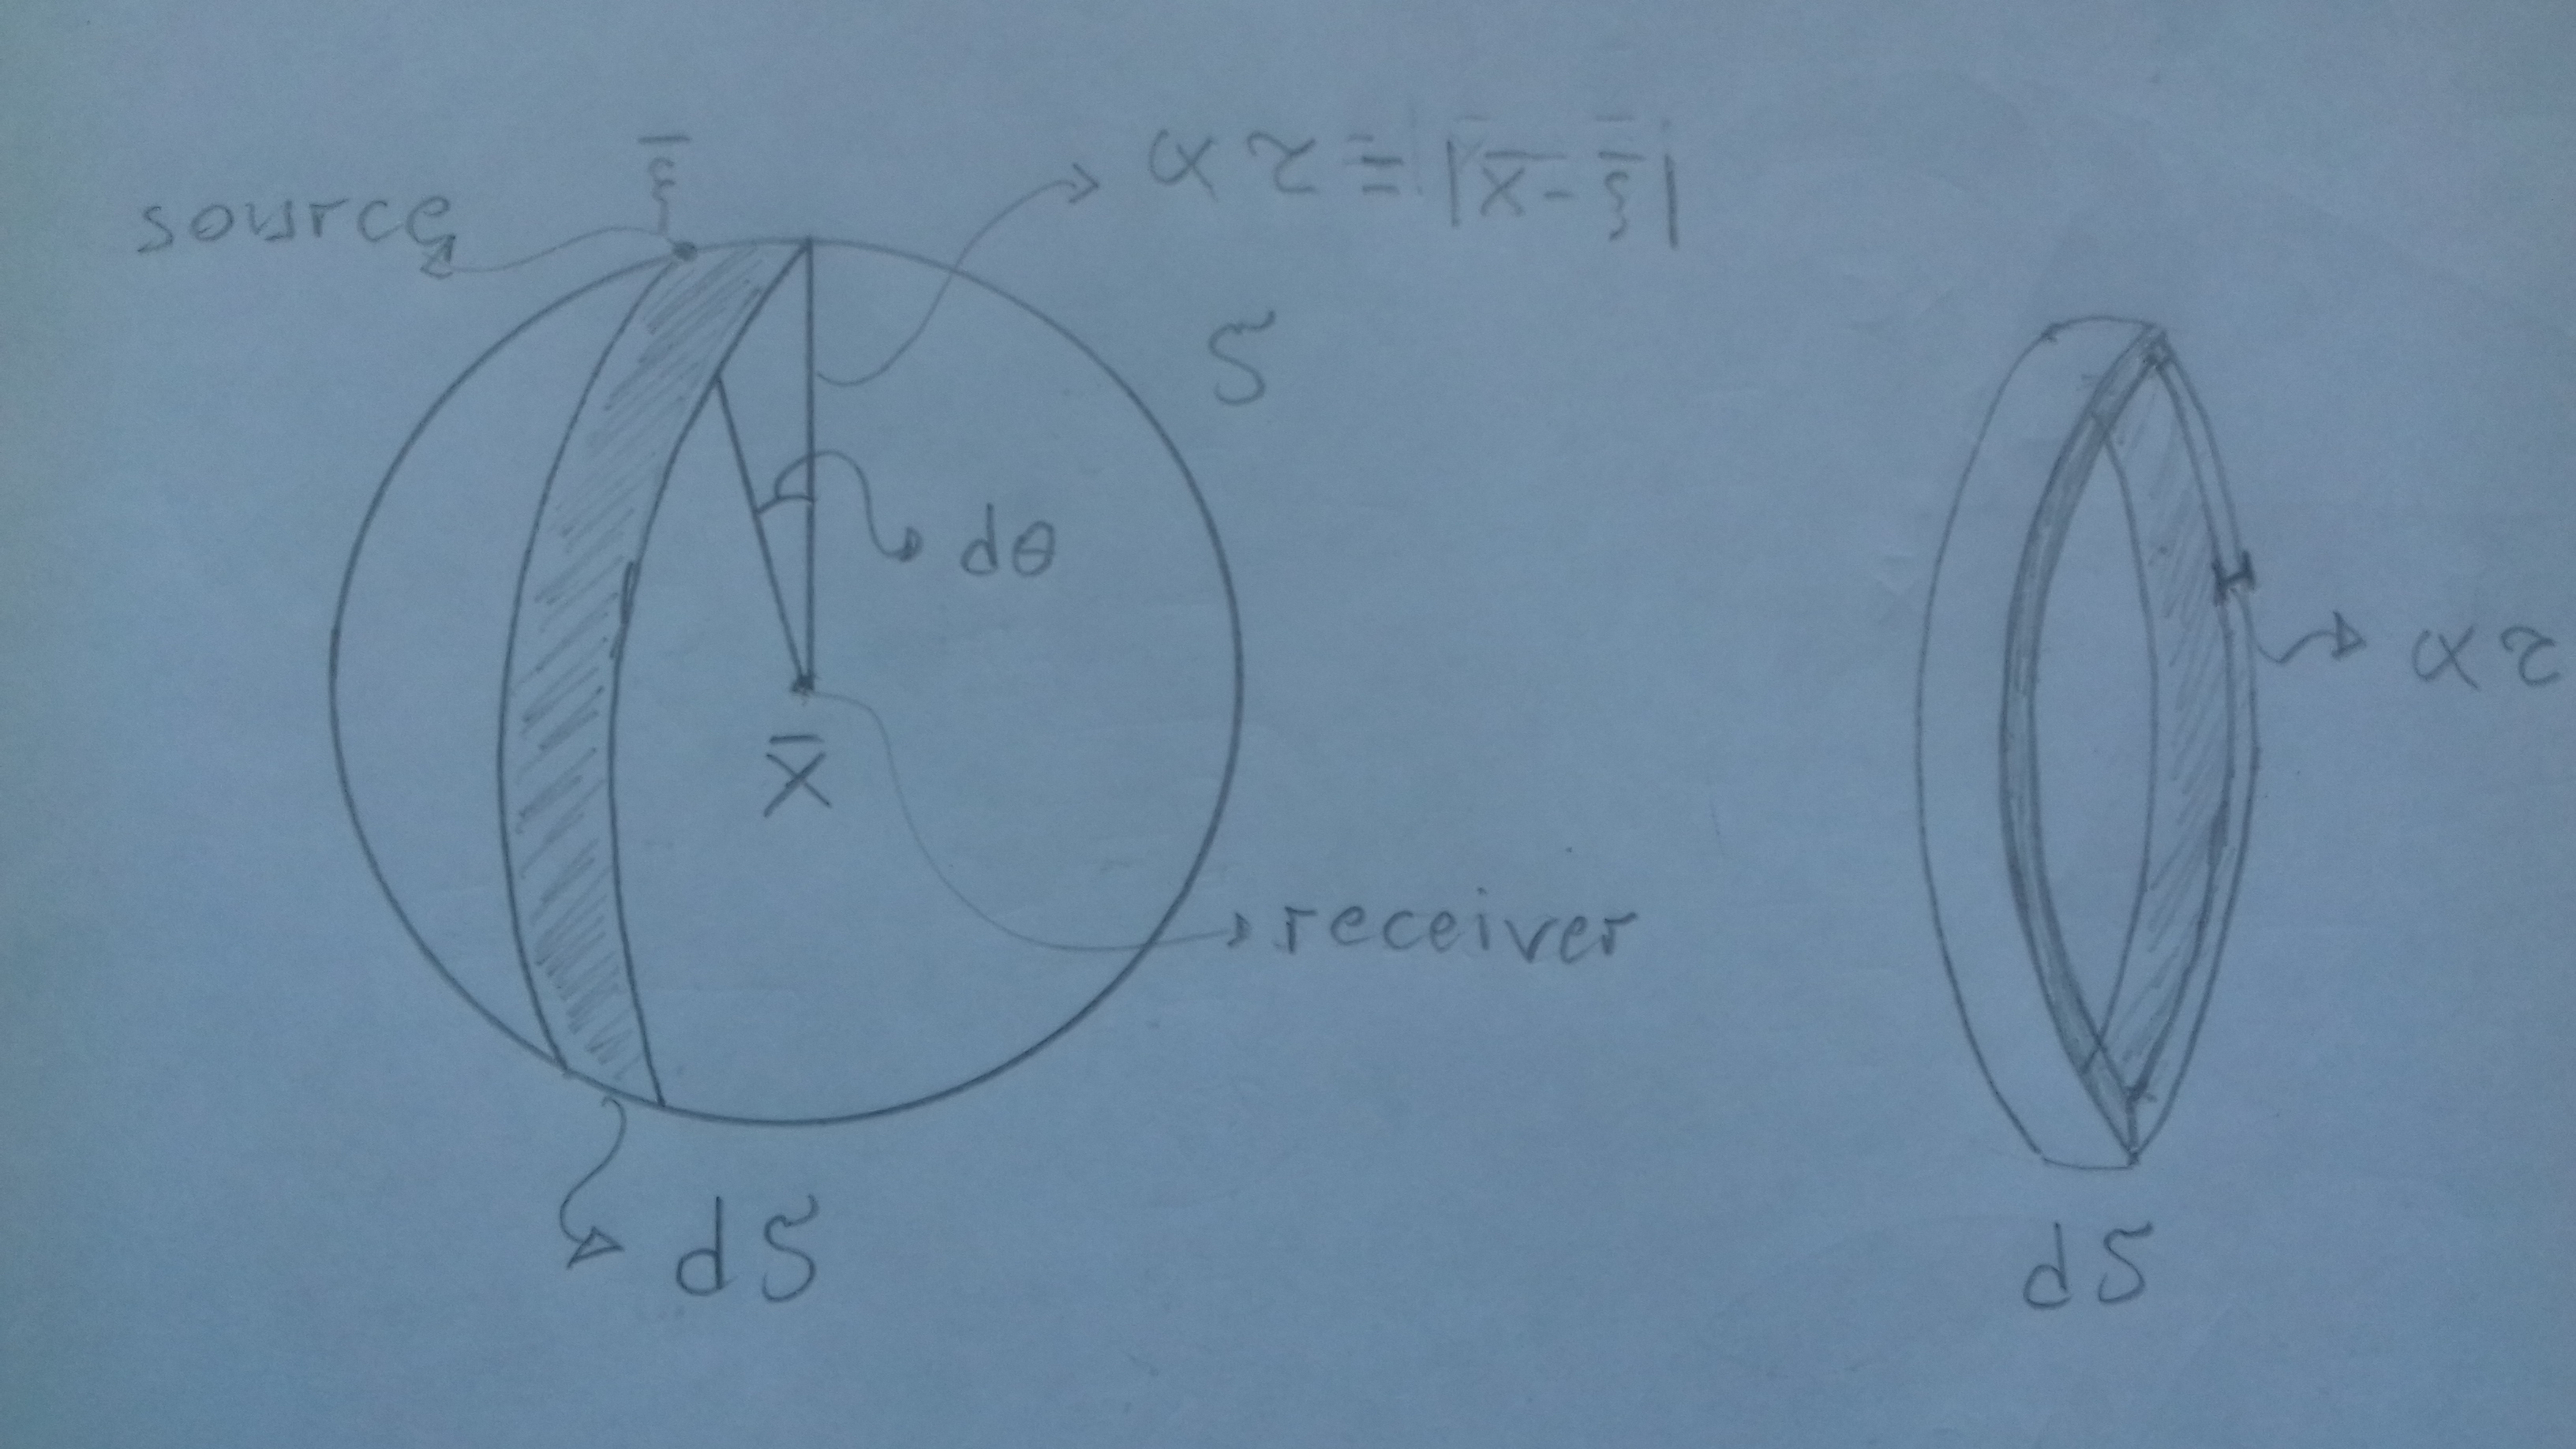
\includegraphics[scale=0.045]{Fig1.jpg}       
			\end{figure}
		\end{column}
	\end{columns}
	
	\begin{flushleft}
		Obtemos a seguinte rela\c{c}\~ao:
	\end{flushleft}
	\begin{eqnarray}
	\int_{V}dV(\eta) &=& \int_{0}^{\infty} \, \alpha \left( \int_{S} dS(\eta) \right) d\tau\, , 
	\end{eqnarray}
	\begin{flushleft}
		onde $\eta$ \'e vari\'avel de integra\c{c}\~ao.
	\end{flushleft}
	
	
\end{frame}%%%%%%%%%%%%%%%%%%%%%%%%%%%%%%%%%%%%%%%%555



\begin{frame}
	\frametitle{\textbf{Solu\c{c}\~ao para a fun\c{c}\~ao de Green em um meio homog\^eneo, isotr\'opico e ilimitado}}
	
	\begin{flushleft}
		\textcolor{red!60!black}{
			Integrando sobre o volume $V$ atrav\'es de um sistema de cascas esf\'ericas conc\^entricas centradas no ponto de observa\c{c}\~ao:}
	\end{flushleft}        
	\begin{eqnarray}
	\int_{V}dV(\eta) &=& \int_{0}^{\infty} \, \alpha \left( \int_{S} dS(\eta) \right) d\tau\, 
	\end{eqnarray}
	
	\begin{flushleft}
		Por compara\c{c}\~ao re-escrevemos:
	\end{flushleft}
	\begin{eqnarray}
	\label{ten1}
	\phi(\xvec,t) &=& - \frac{1}{(4\pi\alpha)^{2} \rho}  \int_{-\infty}^{+\infty}\, d\tau \frac{ X_{0} \left( \xivec,t - \tau  \right) }{\tau}  \int_{S}\frac{\partial }{\partial \xi_1} \frac{1}{\left| \xivec \right|} dS\, \\
	\psi(\xvec,t) &=& \frac{1}{(4\pi\beta)^{2} \rho}  \int_{-\infty}^{+\infty}\, d\tau  \frac{ X_{0}  \left( \xivec,t - \tau  \right) }{\tau}    \int_{S} \left(0, \frac{\partial }{\partial \xi_3} \frac{1}{\left| \xivec \right|}, \frac{\partial }{\partial \xi_2} \frac{1}{\left| \xivec \right|} \right) dS \, \nonumber \\
	\end{eqnarray}
	
\end{frame}%%%%%%%%%%%%%%%%%%%%%%%%%%%%%%%%%%%%%%%%555



\begin{frame}
	\frametitle{\textbf{Solu\c{c}\~ao para a fun\c{c}\~ao de Green em um meio homog\^eneo, isotr\'opico e ilimitado}}
	
	\begin{flushleft}
		Avaliando a integral de superf\'icie:
	\end{flushleft}
	\begin{eqnarray}
	\label{ten1}
	h &=& - \int_{S}\frac{\partial }{\partial \eta_{1}} \frac{1}{R} dS(\eta) \, 
	\end{eqnarray}
	
	\begin{columns}        
		\begin{column}{0.15\textwidth}  
			\begin{eqnarray*}
				\alpha\tau &=& \left| \xvec - \xivec \right|\\
				R &=& \left| \xivec -\eta \right|\\
				r &=&  \left| \xvec - \eta \right|
			\end{eqnarray*}
		\end{column}
		\begin{column}{0.75\textwidth}    
			\begin{figure}[h!]   
				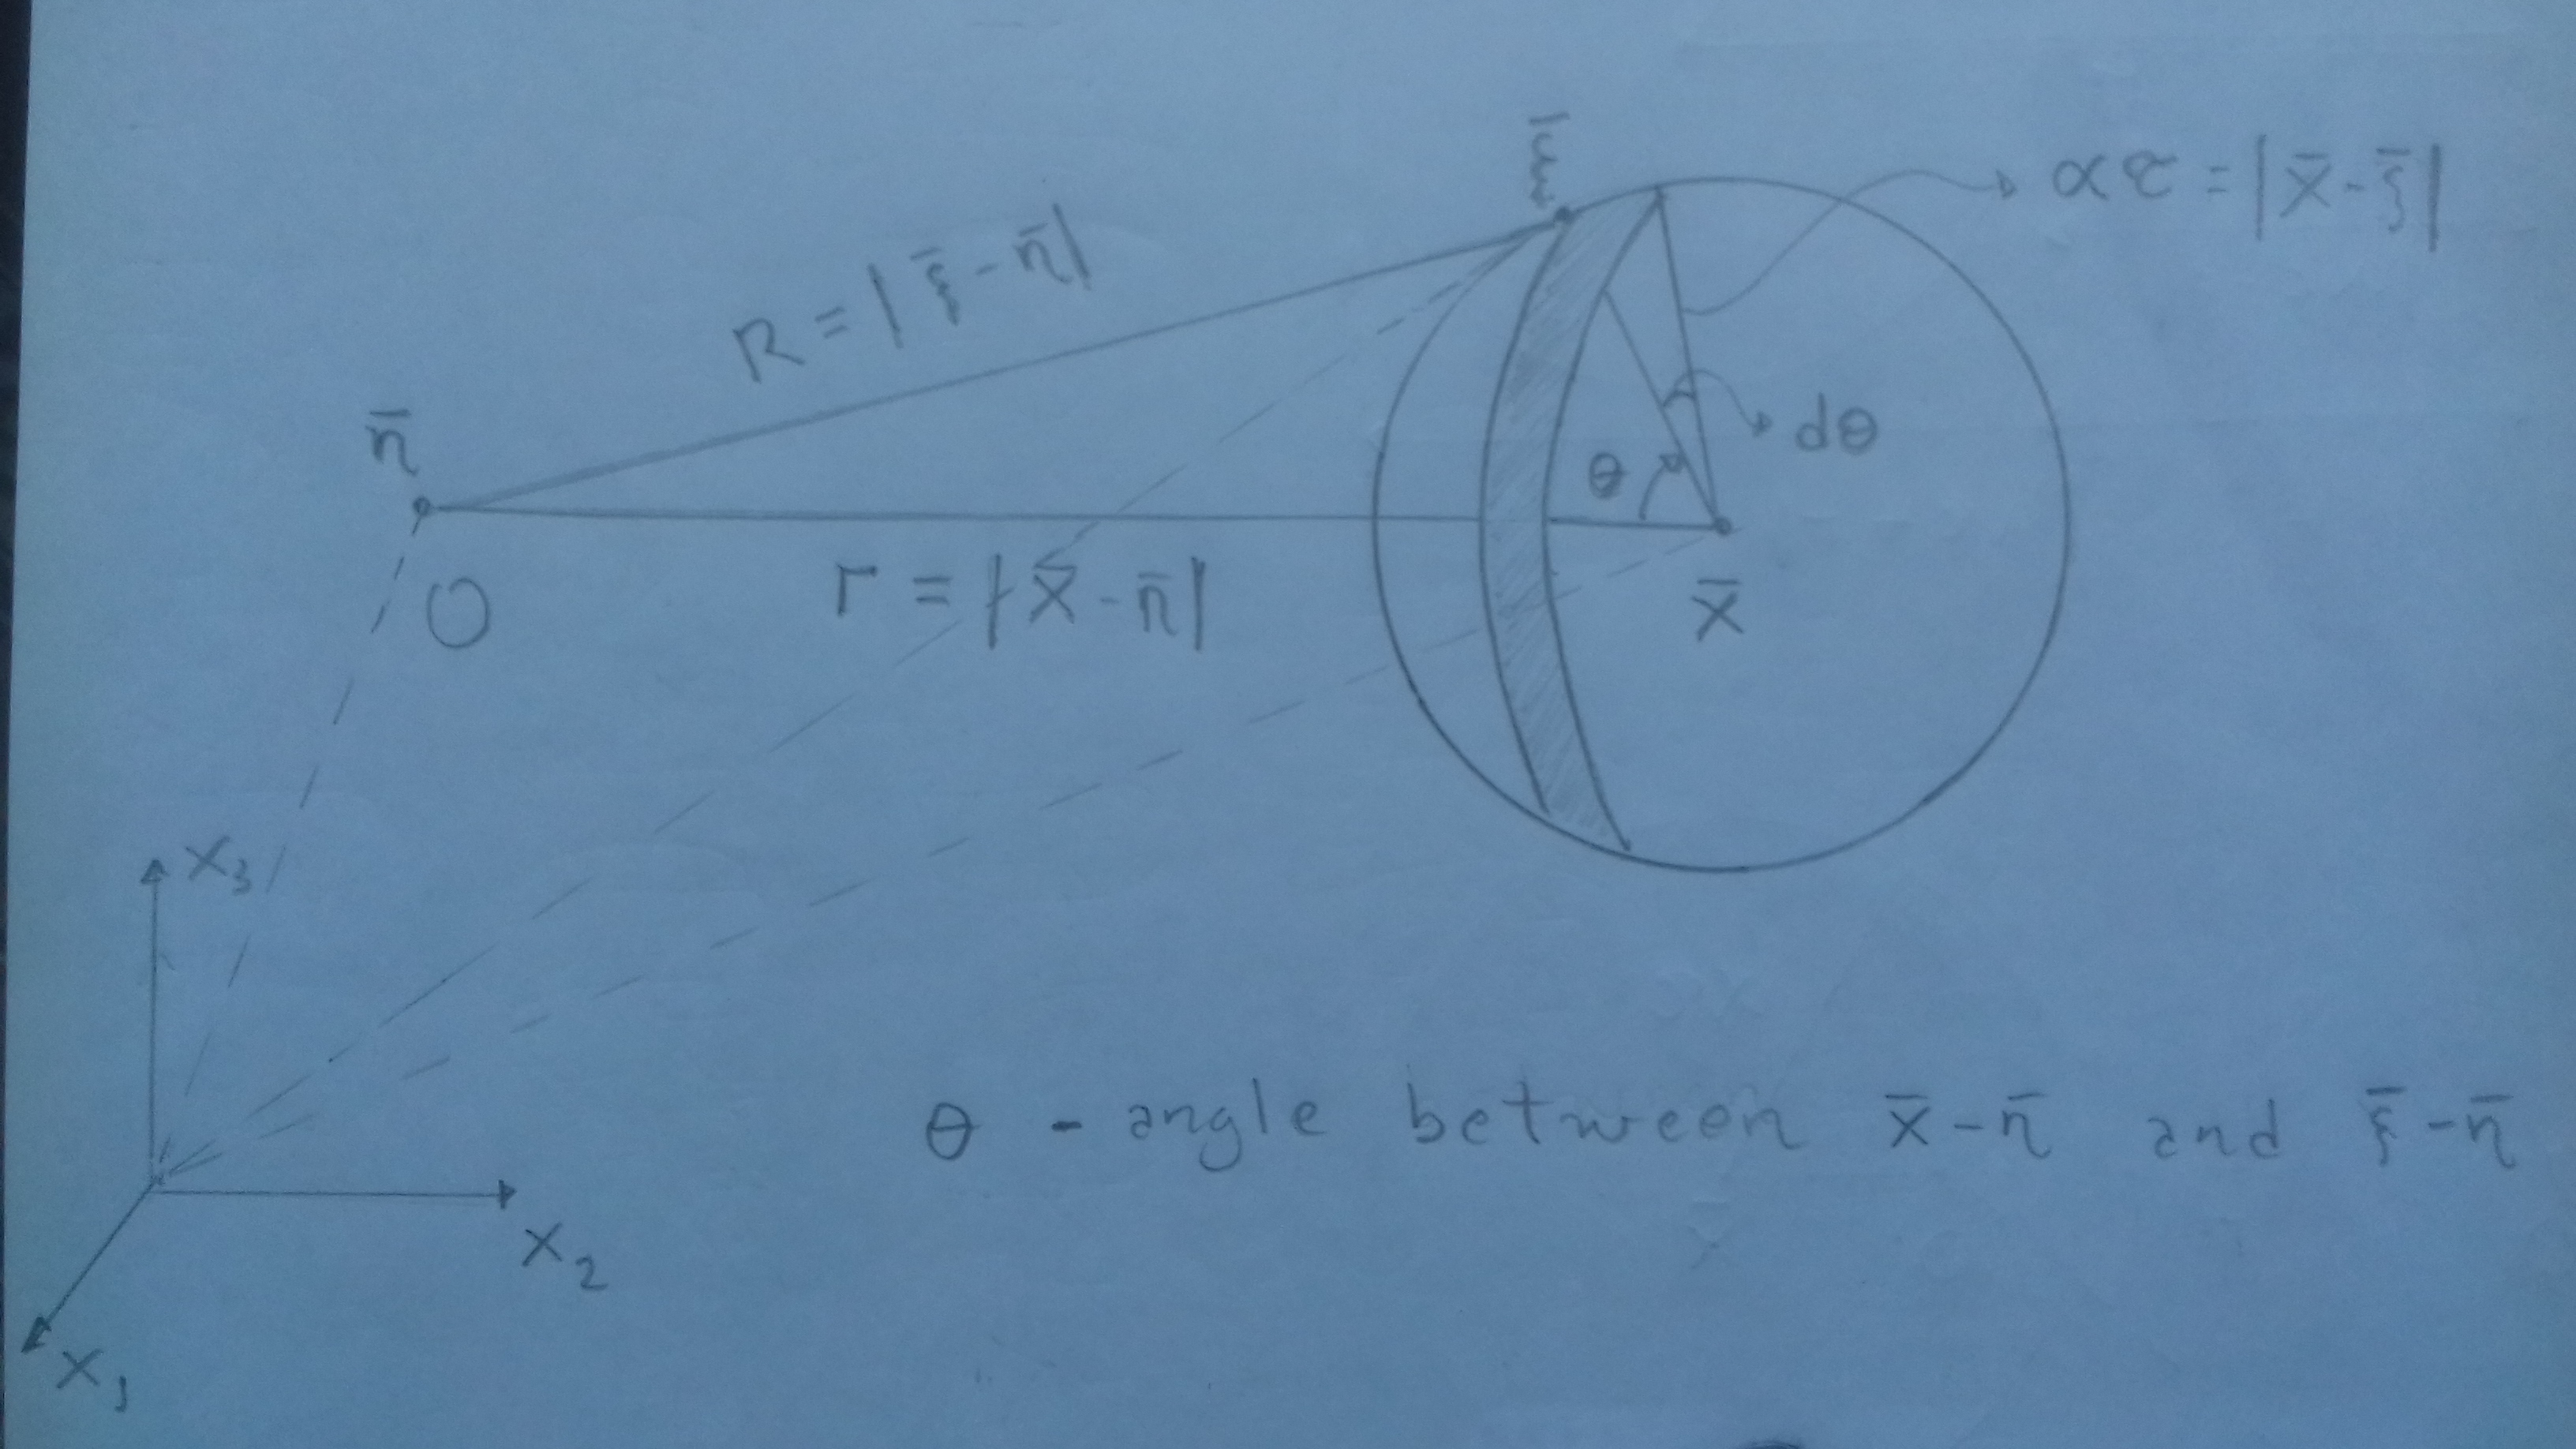
\includegraphics[width=248px, height=120px]{Fig11.jpg}     
			\end{figure}
		\end{column}
	\end{columns}
	
\end{frame}%%%%%%%%%%%%%%%%%%%%%%%%%%%%%%%%%%%%%%%%555


\begin{frame}
	\frametitle{\textbf{Solu\c{c}\~ao para a fun\c{c}\~ao de Green em um meio homog\^eneo, isotr\'opico e ilimitado}}
	
	\begin{flushleft}
		\textcolor{red!60!black}{Avaliando a integral de superf\'icie:}
	\end{flushleft}
	
	\begin{figure}[h!]   
		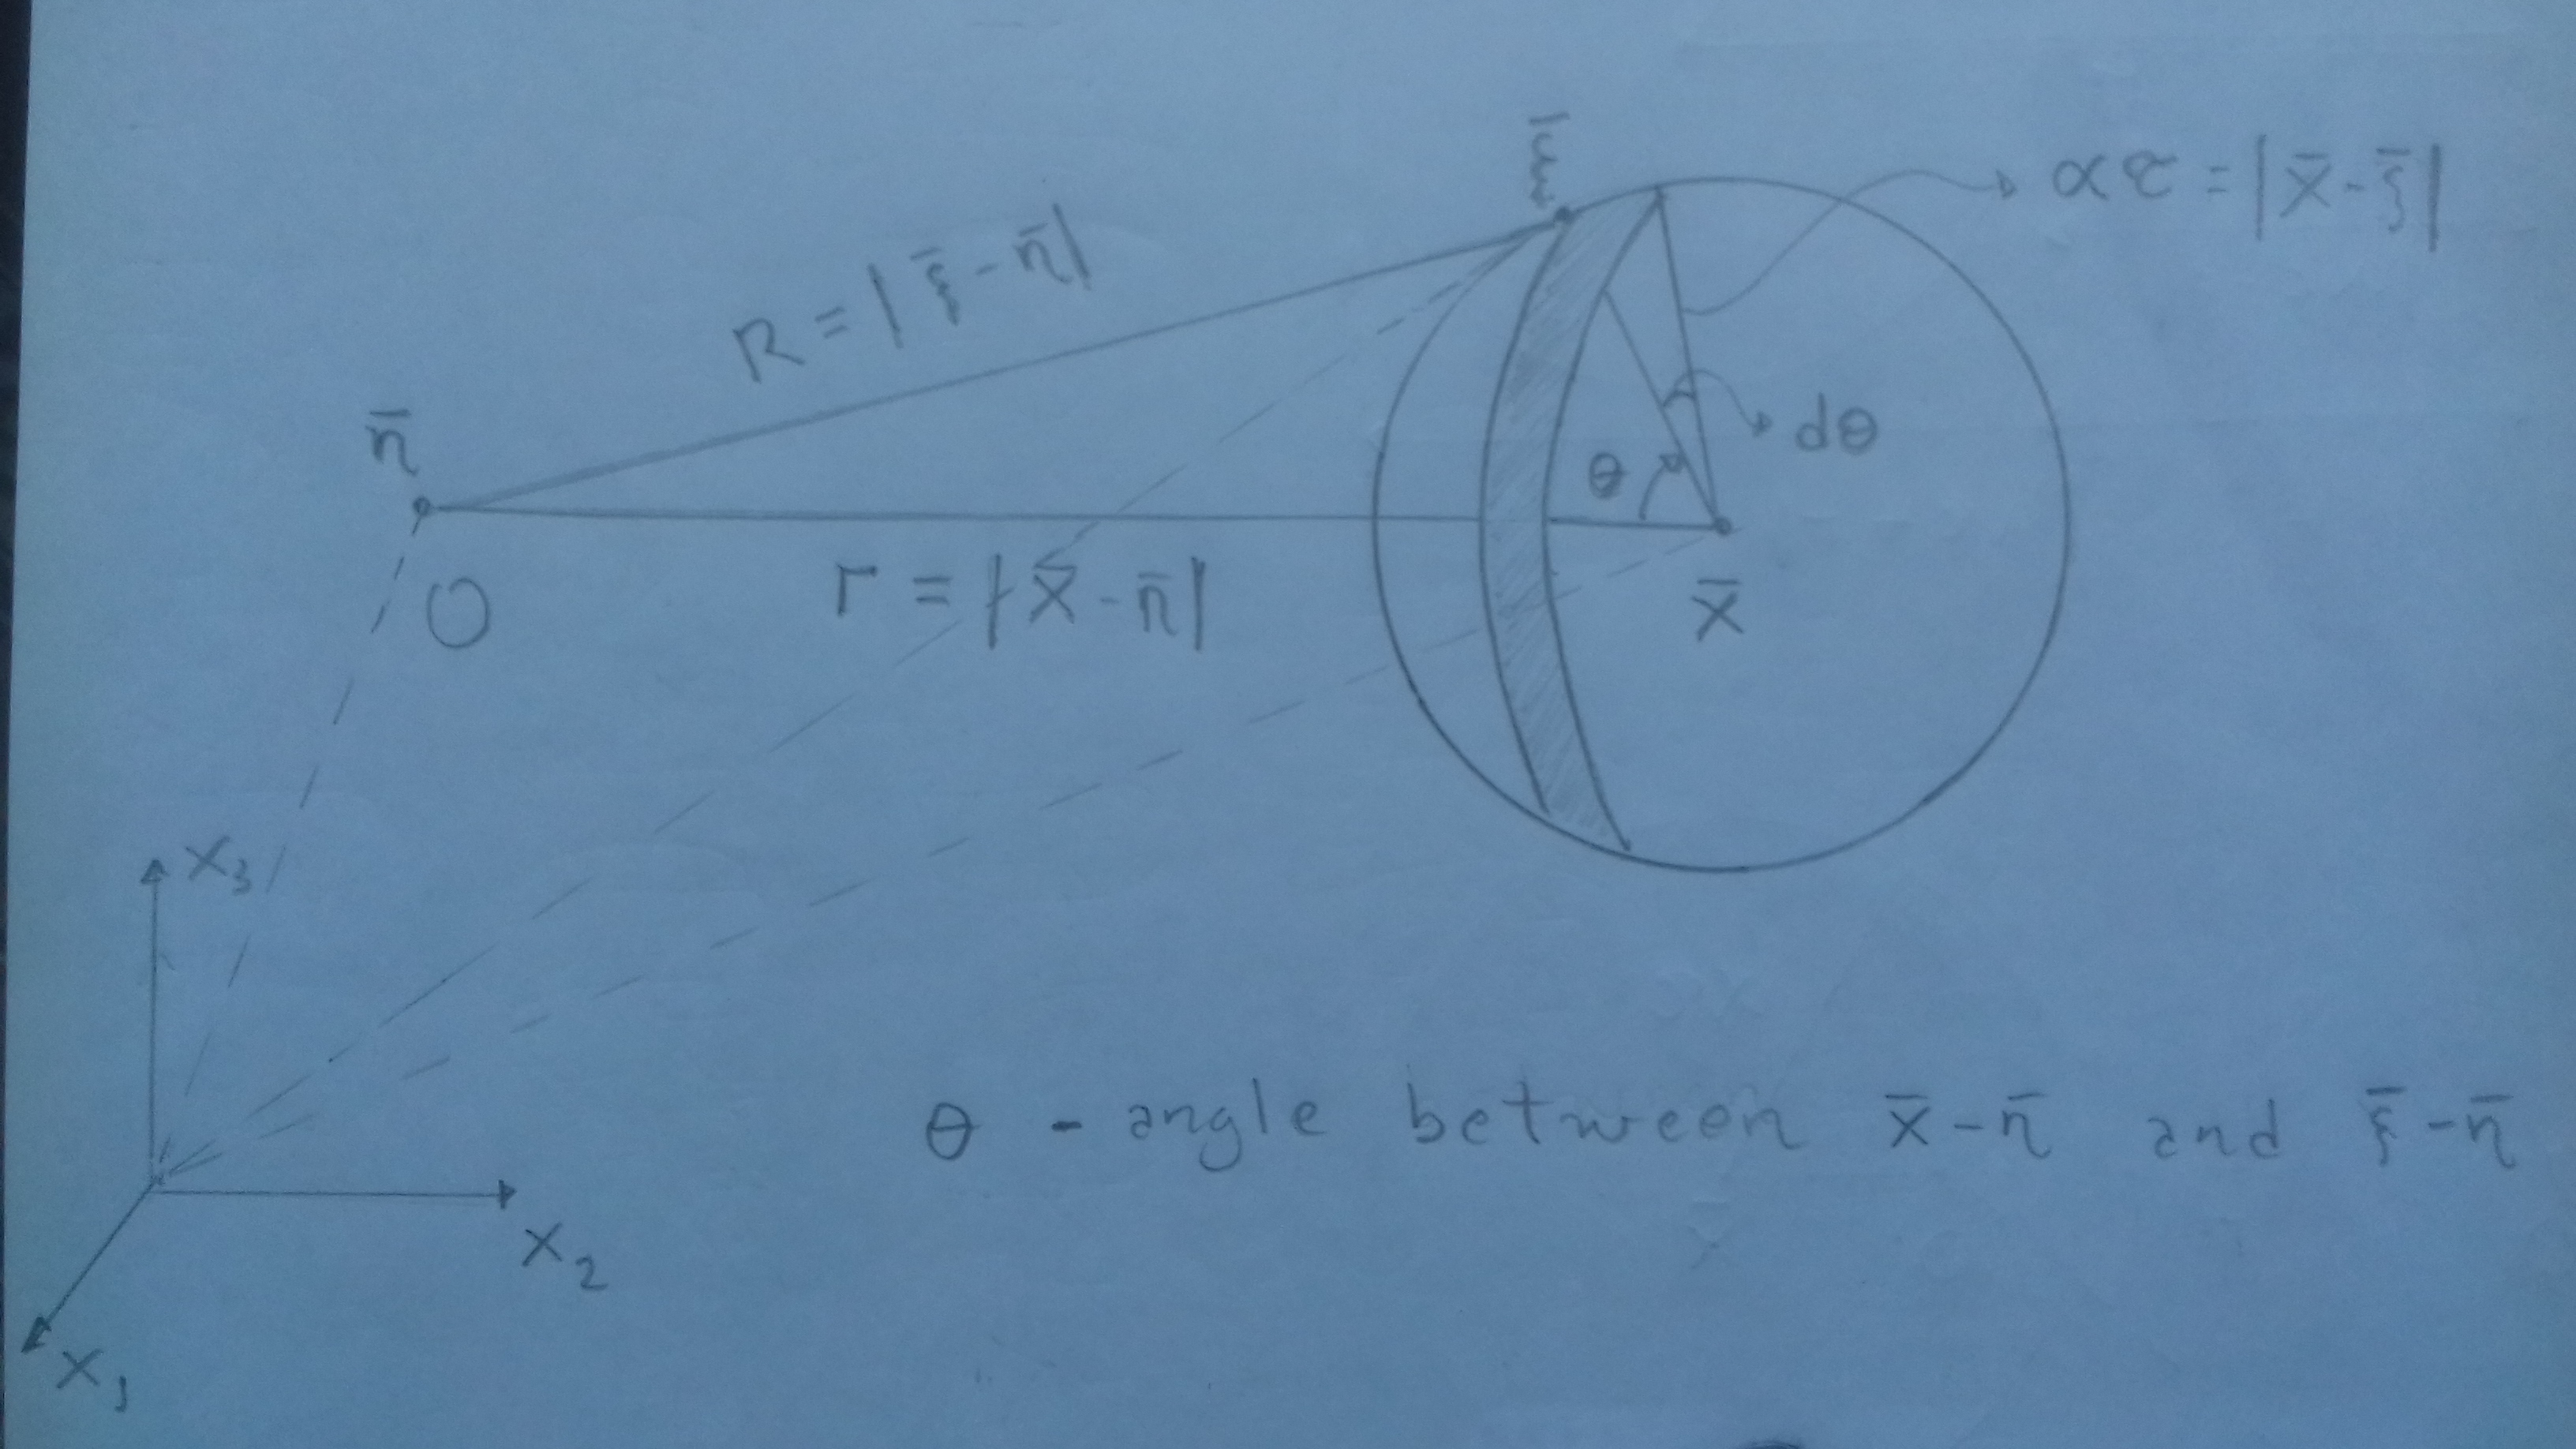
\includegraphics[width=218px, height=100px]{Fig11.jpg}       
	\end{figure}
	\begin{flushleft}
		A vari\'avel integra\c{c}\~ao $\eta$ \'e fixa para todos os pontos $\xivec$ em $S$, 
	\end{flushleft}
	\begin{eqnarray}
	\label{ten1}
	h &=& - \int_{S}\frac{\partial }{\partial \eta_{1}} \frac{1}{R} dS(\eta)  = - \frac{\partial }{\partial \eta_{1}}\int_{S} \frac{1}{R} dS(\eta) \, 
	\end{eqnarray}
	
\end{frame}%%%%%%%%%%%%%%%%%%%%%%%%%%%%%%%%%%%%%%%%555


%\begin{frame}
%	\frametitle{\textbf{Solu\c{c}\~ao para a fun\c{c}\~ao de Green em um meio homog\^eneo, isotr\'opico e ilimitado}}
%%	\begin{flushleft}
%%		\textcolor{red!60!black}{Avaliando a integral de superf\'icie:}
%%	\end{flushleft}    
%	
%	\begin{figure}[h!]   
%		\begin{subfigure}[t]{0.40\linewidth}
%			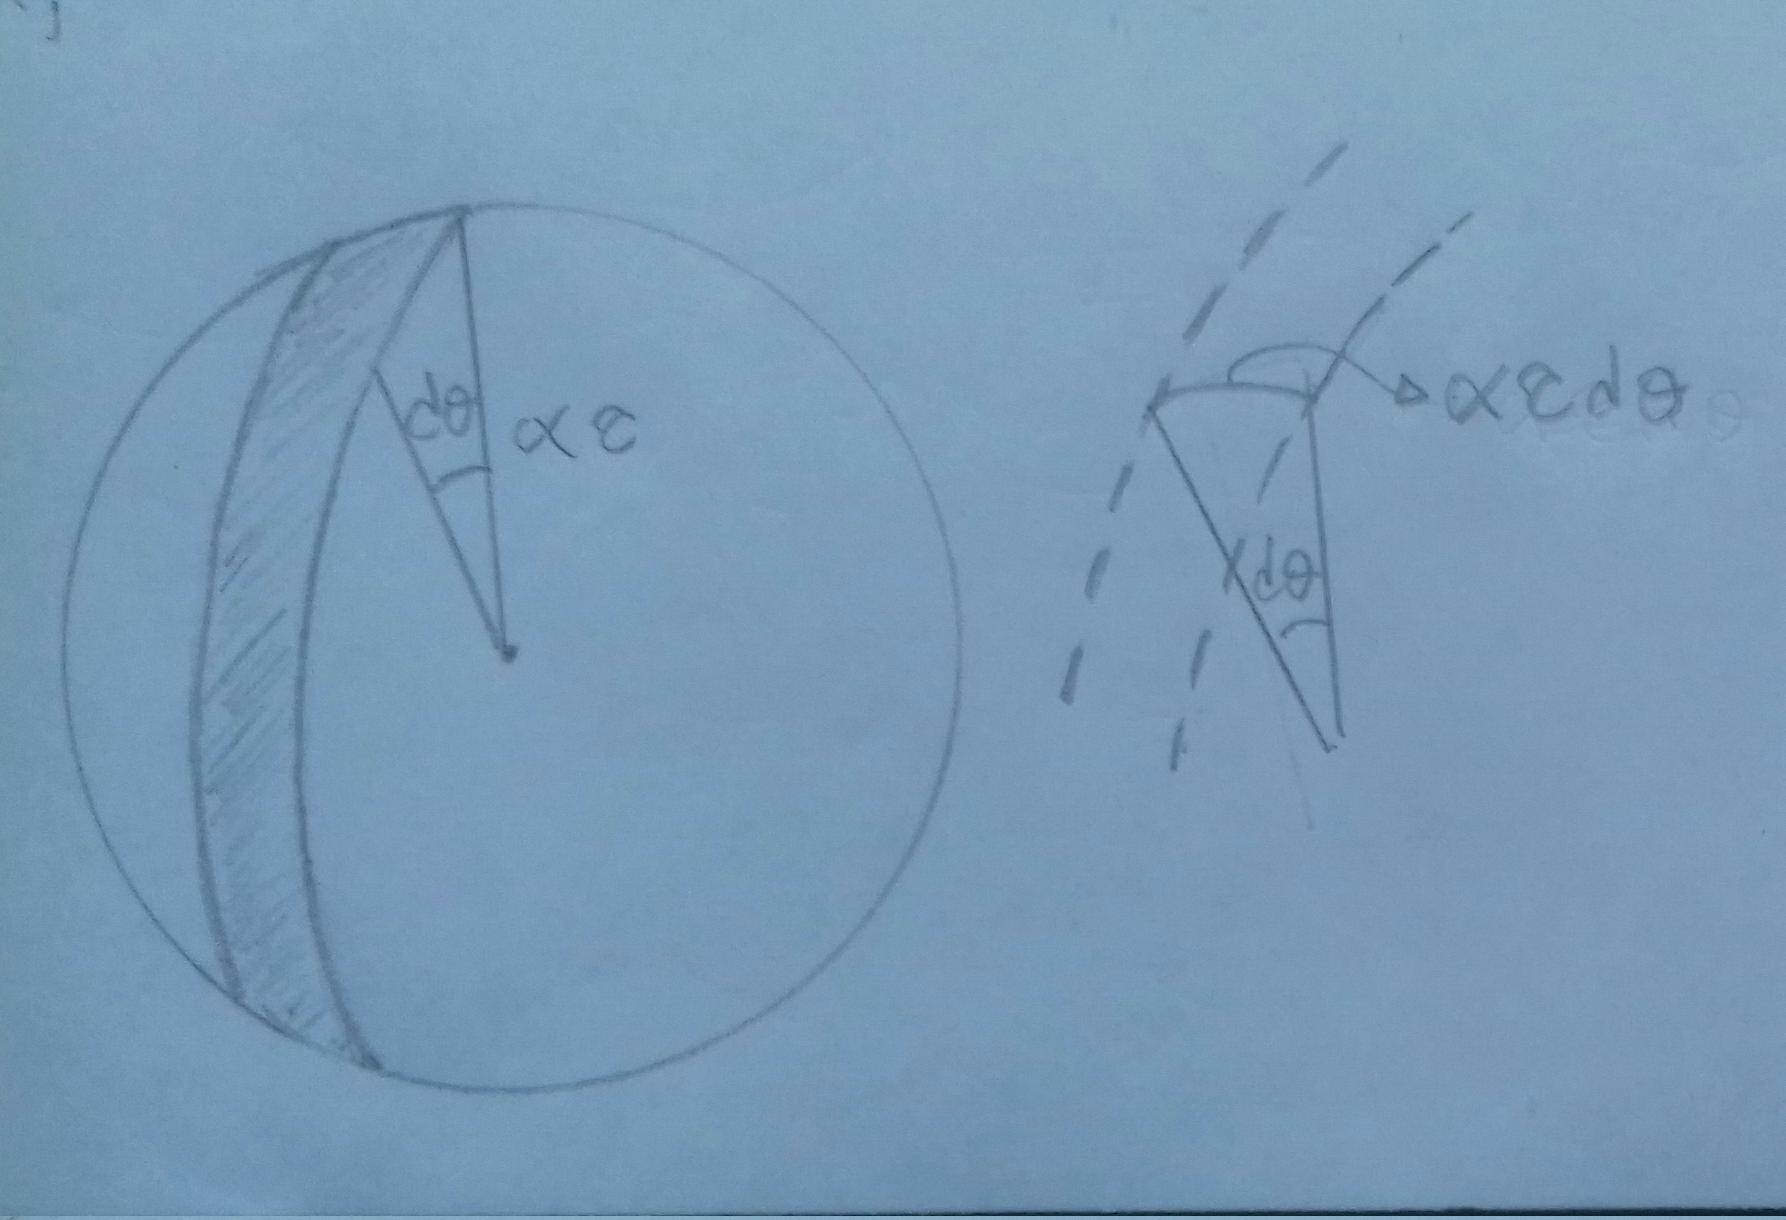
\includegraphics[scale=0.060]{Fig3.jpg}\\        
%		\end{subfigure}  
%		\begin{subfigure}[t]{0.40\linewidth}
%			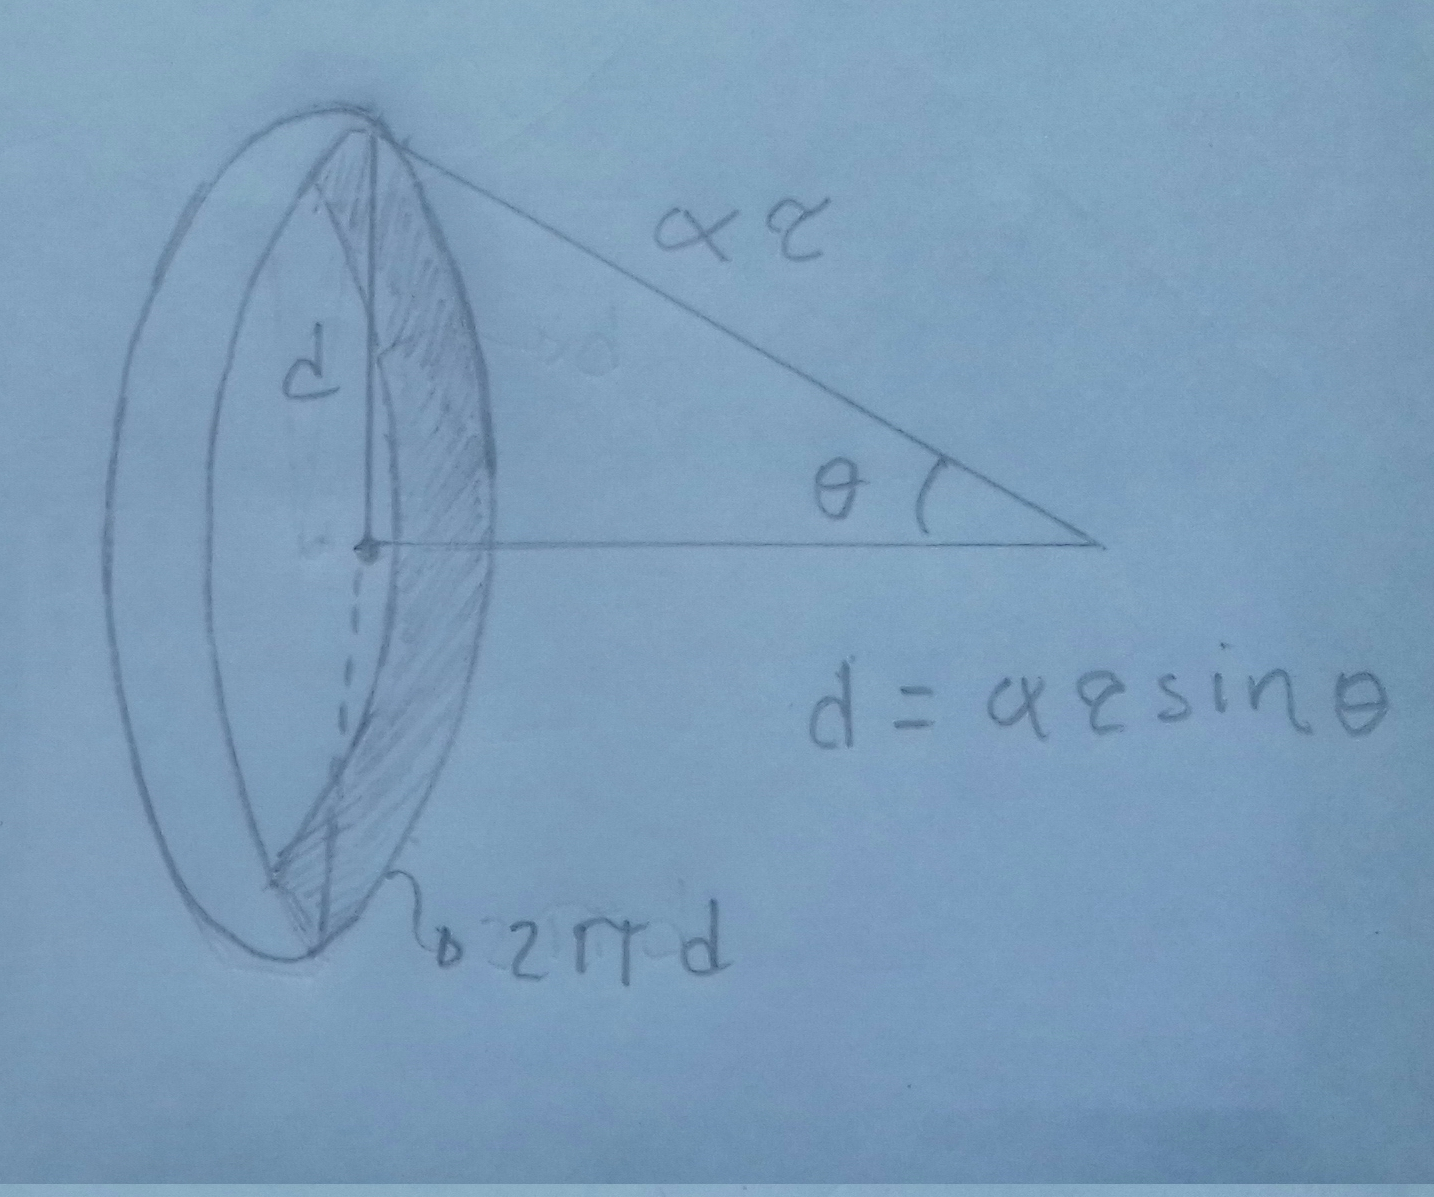
\includegraphics[scale=0.0615]{Fig4.jpg}\\            
%		\end{subfigure}    
%	\end{figure}  
%	\begin{flushleft}
%		Um elemento de superf\'icie $dS$ \'e 
%	\end{flushleft}
%	\begin{eqnarray}
%	\label{ten1}
%	dS &=& 2\pi \alpha^2 \tau^2 \sin \theta d\theta \, .
%	\end{eqnarray}
%	\begin{flushleft}
%		Substituindo o elemento de superf\'icie $dS$,
%	\end{flushleft}
%	\begin{eqnarray}
%	\label{ten1}
%	\int_{S} \frac{1}{R} dS(\eta)  &=& 2\pi \alpha^2 \tau^2 \int_{0}^{\pi} \frac{\sin \theta}{R} d\theta \, 
%	\end{eqnarray}
%	
%\end{frame}%%%%%%%%%%%%%%%%%%%%%%%%%%%%%%%%%%%%%%%%555



\begin{frame}
	\frametitle{\textbf{Solu\c{c}\~ao para a fun\c{c}\~ao de Green em um meio homog\^eneo, isotr\'opico e ilimitado}}
	\begin{flushleft}
		\textcolor{red!60!black}{Avaliando a integral de superf\'icie:}
	\end{flushleft}
	
	\begin{columns}        
		\begin{column}{0.60\textwidth}  
			\begin{figure}[h!]   
				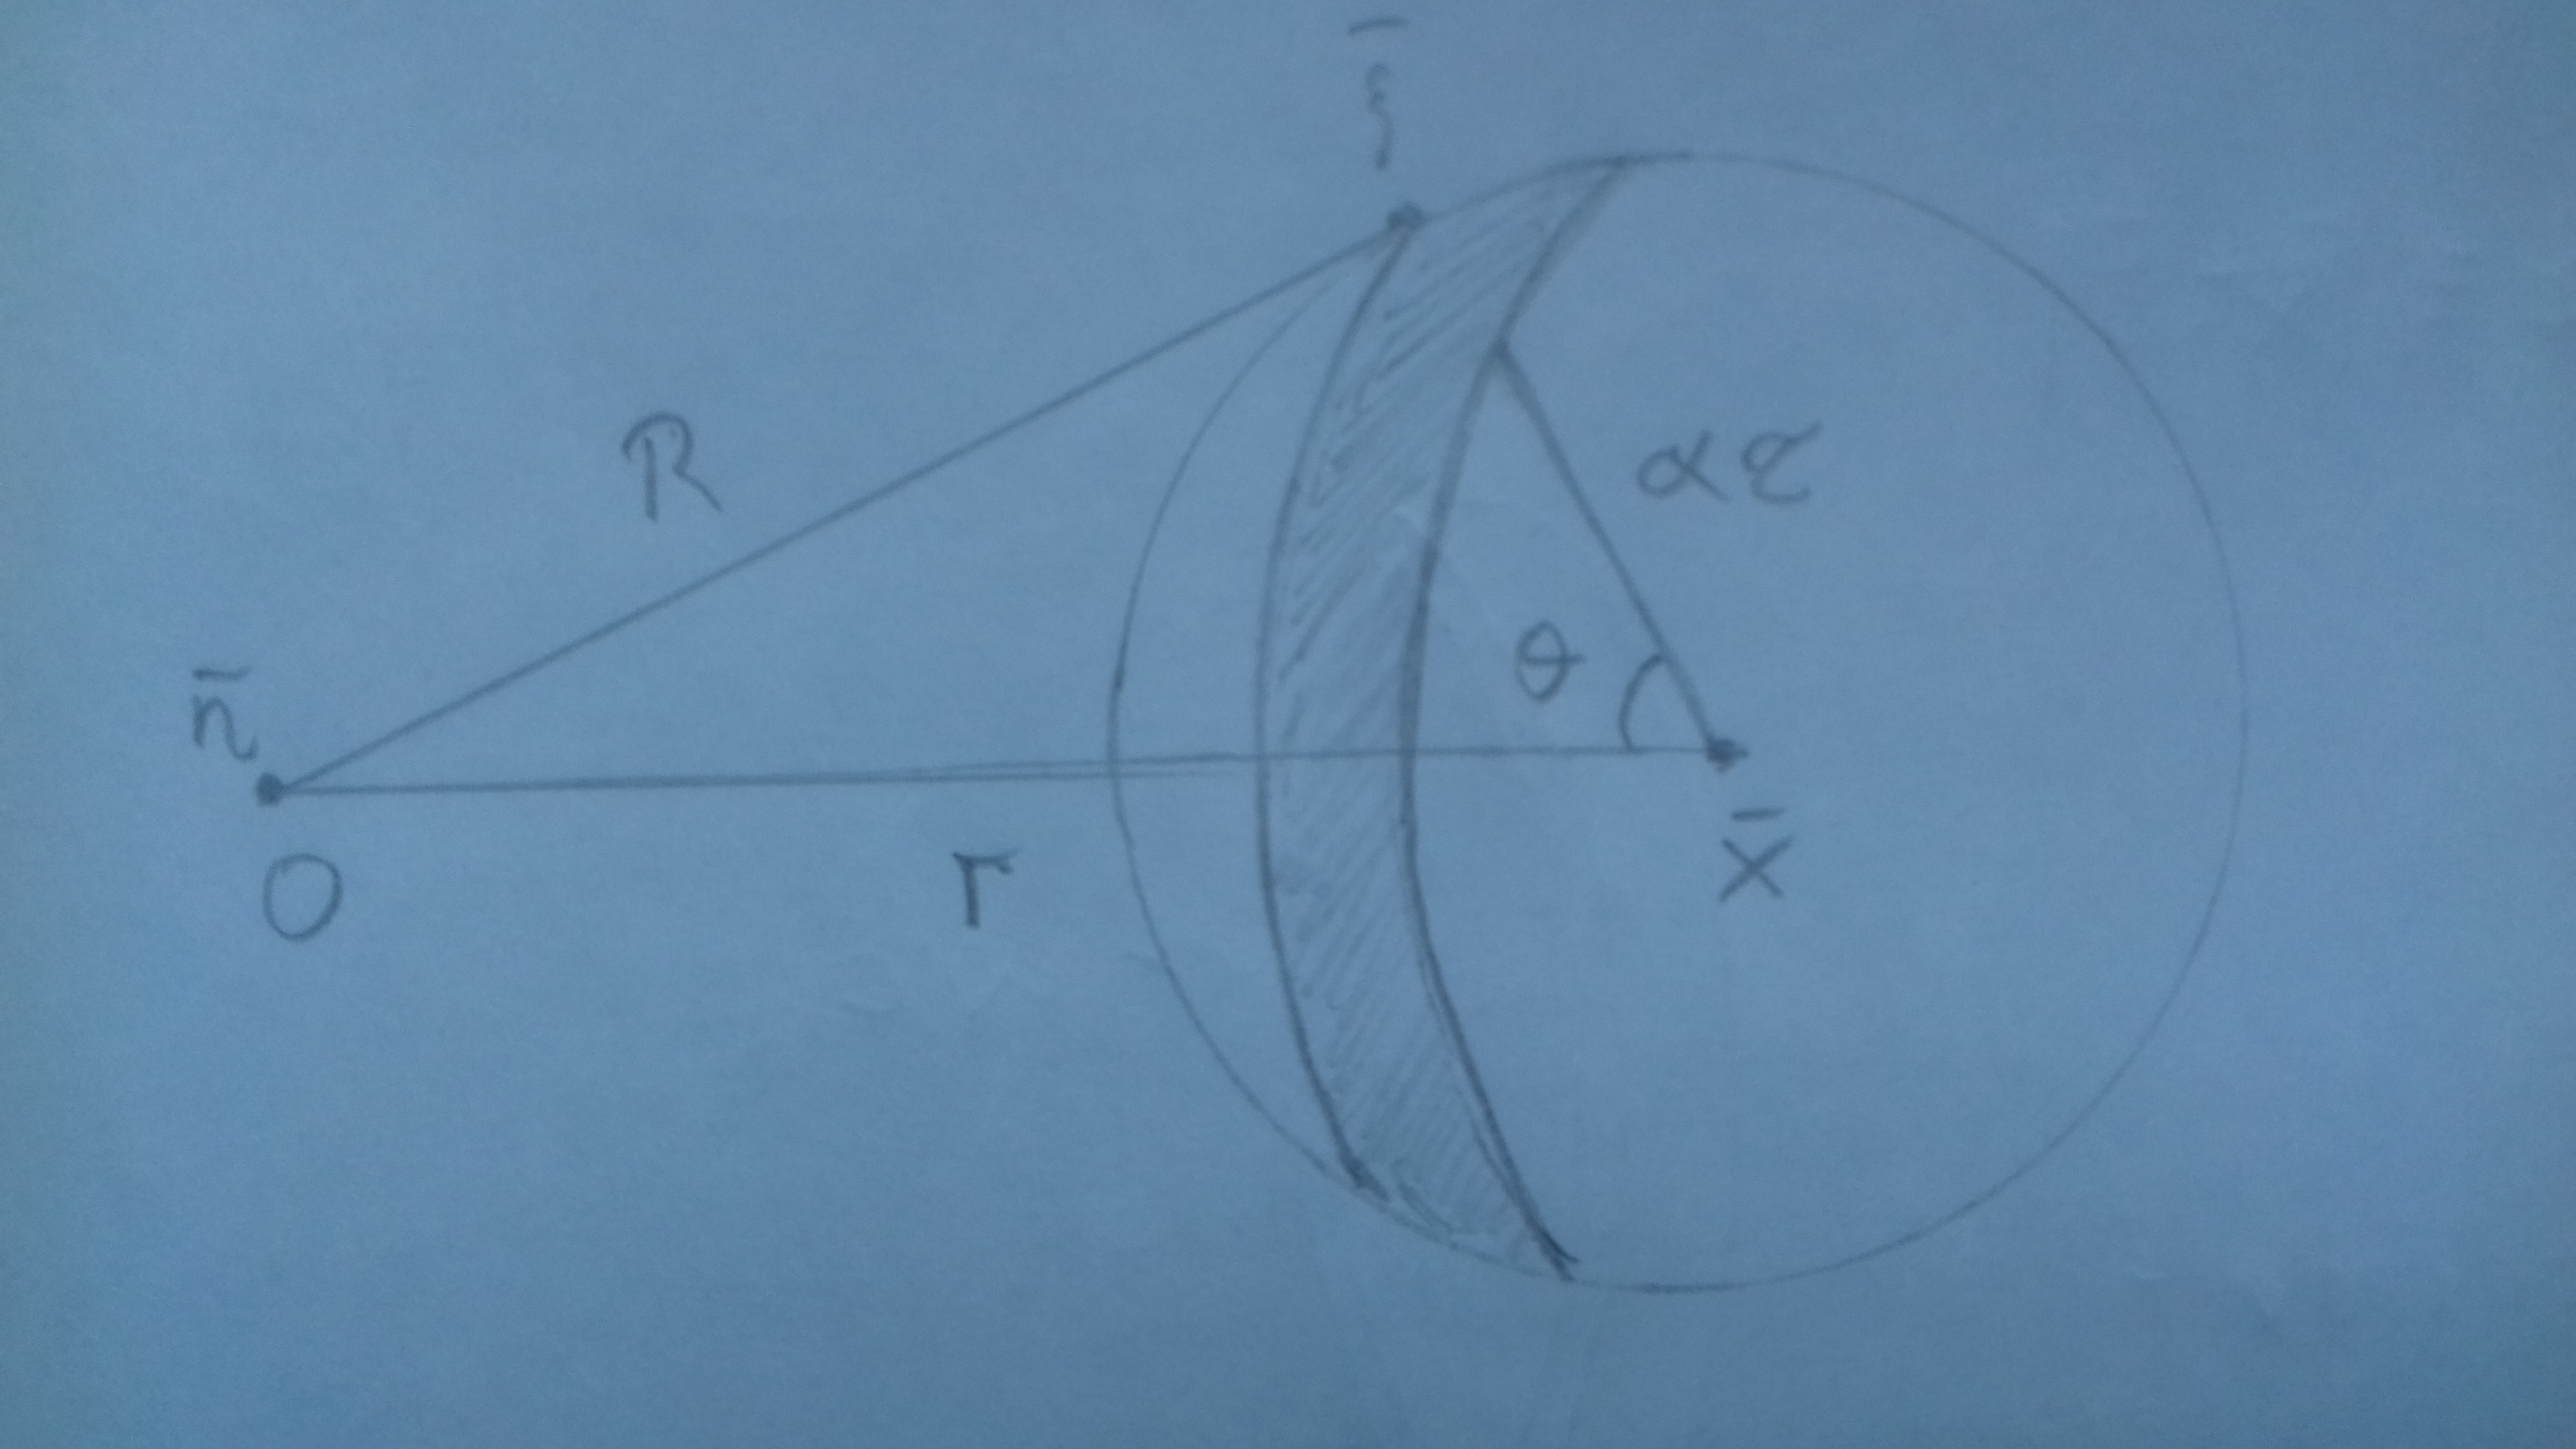
\includegraphics[scale=0.058]{Fig5.jpg}       
			\end{figure}
		\end{column}
	\end{columns}
	
	\begin{flushleft}
		A express\~ao para $\sin \theta d\theta$ usando a lei dos cosenos,
	\end{flushleft}
	\begin{eqnarray}
	\label{ten1}
	R &=&  r^2 + \alpha^2 \tau^2  - 2r\alpha\tau \cos \theta\,
	\end{eqnarray}
	
\end{frame}%%%%%%%%%%%%%%%%%%%%%%%%%%%%%%%%%%%%%%%%555


\begin{frame}
	\frametitle{\textbf{Solu\c{c}\~ao para a fun\c{c}\~ao de Green em um meio homog\^eneo, isotr\'opico e ilimitado}}
	\begin{flushleft}
		\textcolor{red!60!black}{Avaliando a integral de superf\'icie:}
	\end{flushleft}
	
	\begin{flushleft}
		A express\~ao para $\sin \theta d\theta$ usando a lei dos cosenos,
	\end{flushleft}
	\begin{eqnarray}
	\label{ten1}
	R &=&  r^2 + \alpha^2 \tau^2  - 2r\alpha\tau \cos \theta\,
	\end{eqnarray}
	\begin{flushleft}
		e tomando o diferencial,
	\end{flushleft}
	\begin{eqnarray}
	\label{ten1}
	2RdR &=& 2r\alpha\tau \sin \theta d\theta \, .
	\end{eqnarray}
	\begin{flushleft}
		Substituindo $\sin \theta d\theta$,
	\end{flushleft}
	\begin{eqnarray}
	\label{ten1}
	\int_{S} \frac{1}{R} dS(\eta)  &=& 2\pi \alpha^2 \tau^2 \int_{0}^{\pi} \frac{\sin \theta}{R} d\theta  = \frac{2\pi \alpha \tau}{r} \int_{\left| \alpha\tau -r \right|}^{\left| \alpha\tau +r \right|}  dR \, 
	\end{eqnarray}
	
\end{frame}%%%%%%%%%%%%%%%%%%%%%%%%%%%%%%%%%%%%%%%%555



\begin{frame}
	\frametitle{\textbf{Solu\c{c}\~ao para a fun\c{c}\~ao de Green em um meio homog\^eneo, isotr\'opico e ilimitado}}
	\begin{flushleft}
		\textcolor{red!60!black}{Avaliando a integral de superf\'icie:}
	\end{flushleft}
	\begin{columns}        
		\begin{column}{0.60\textwidth}    
			\begin{figure}[h!]   
				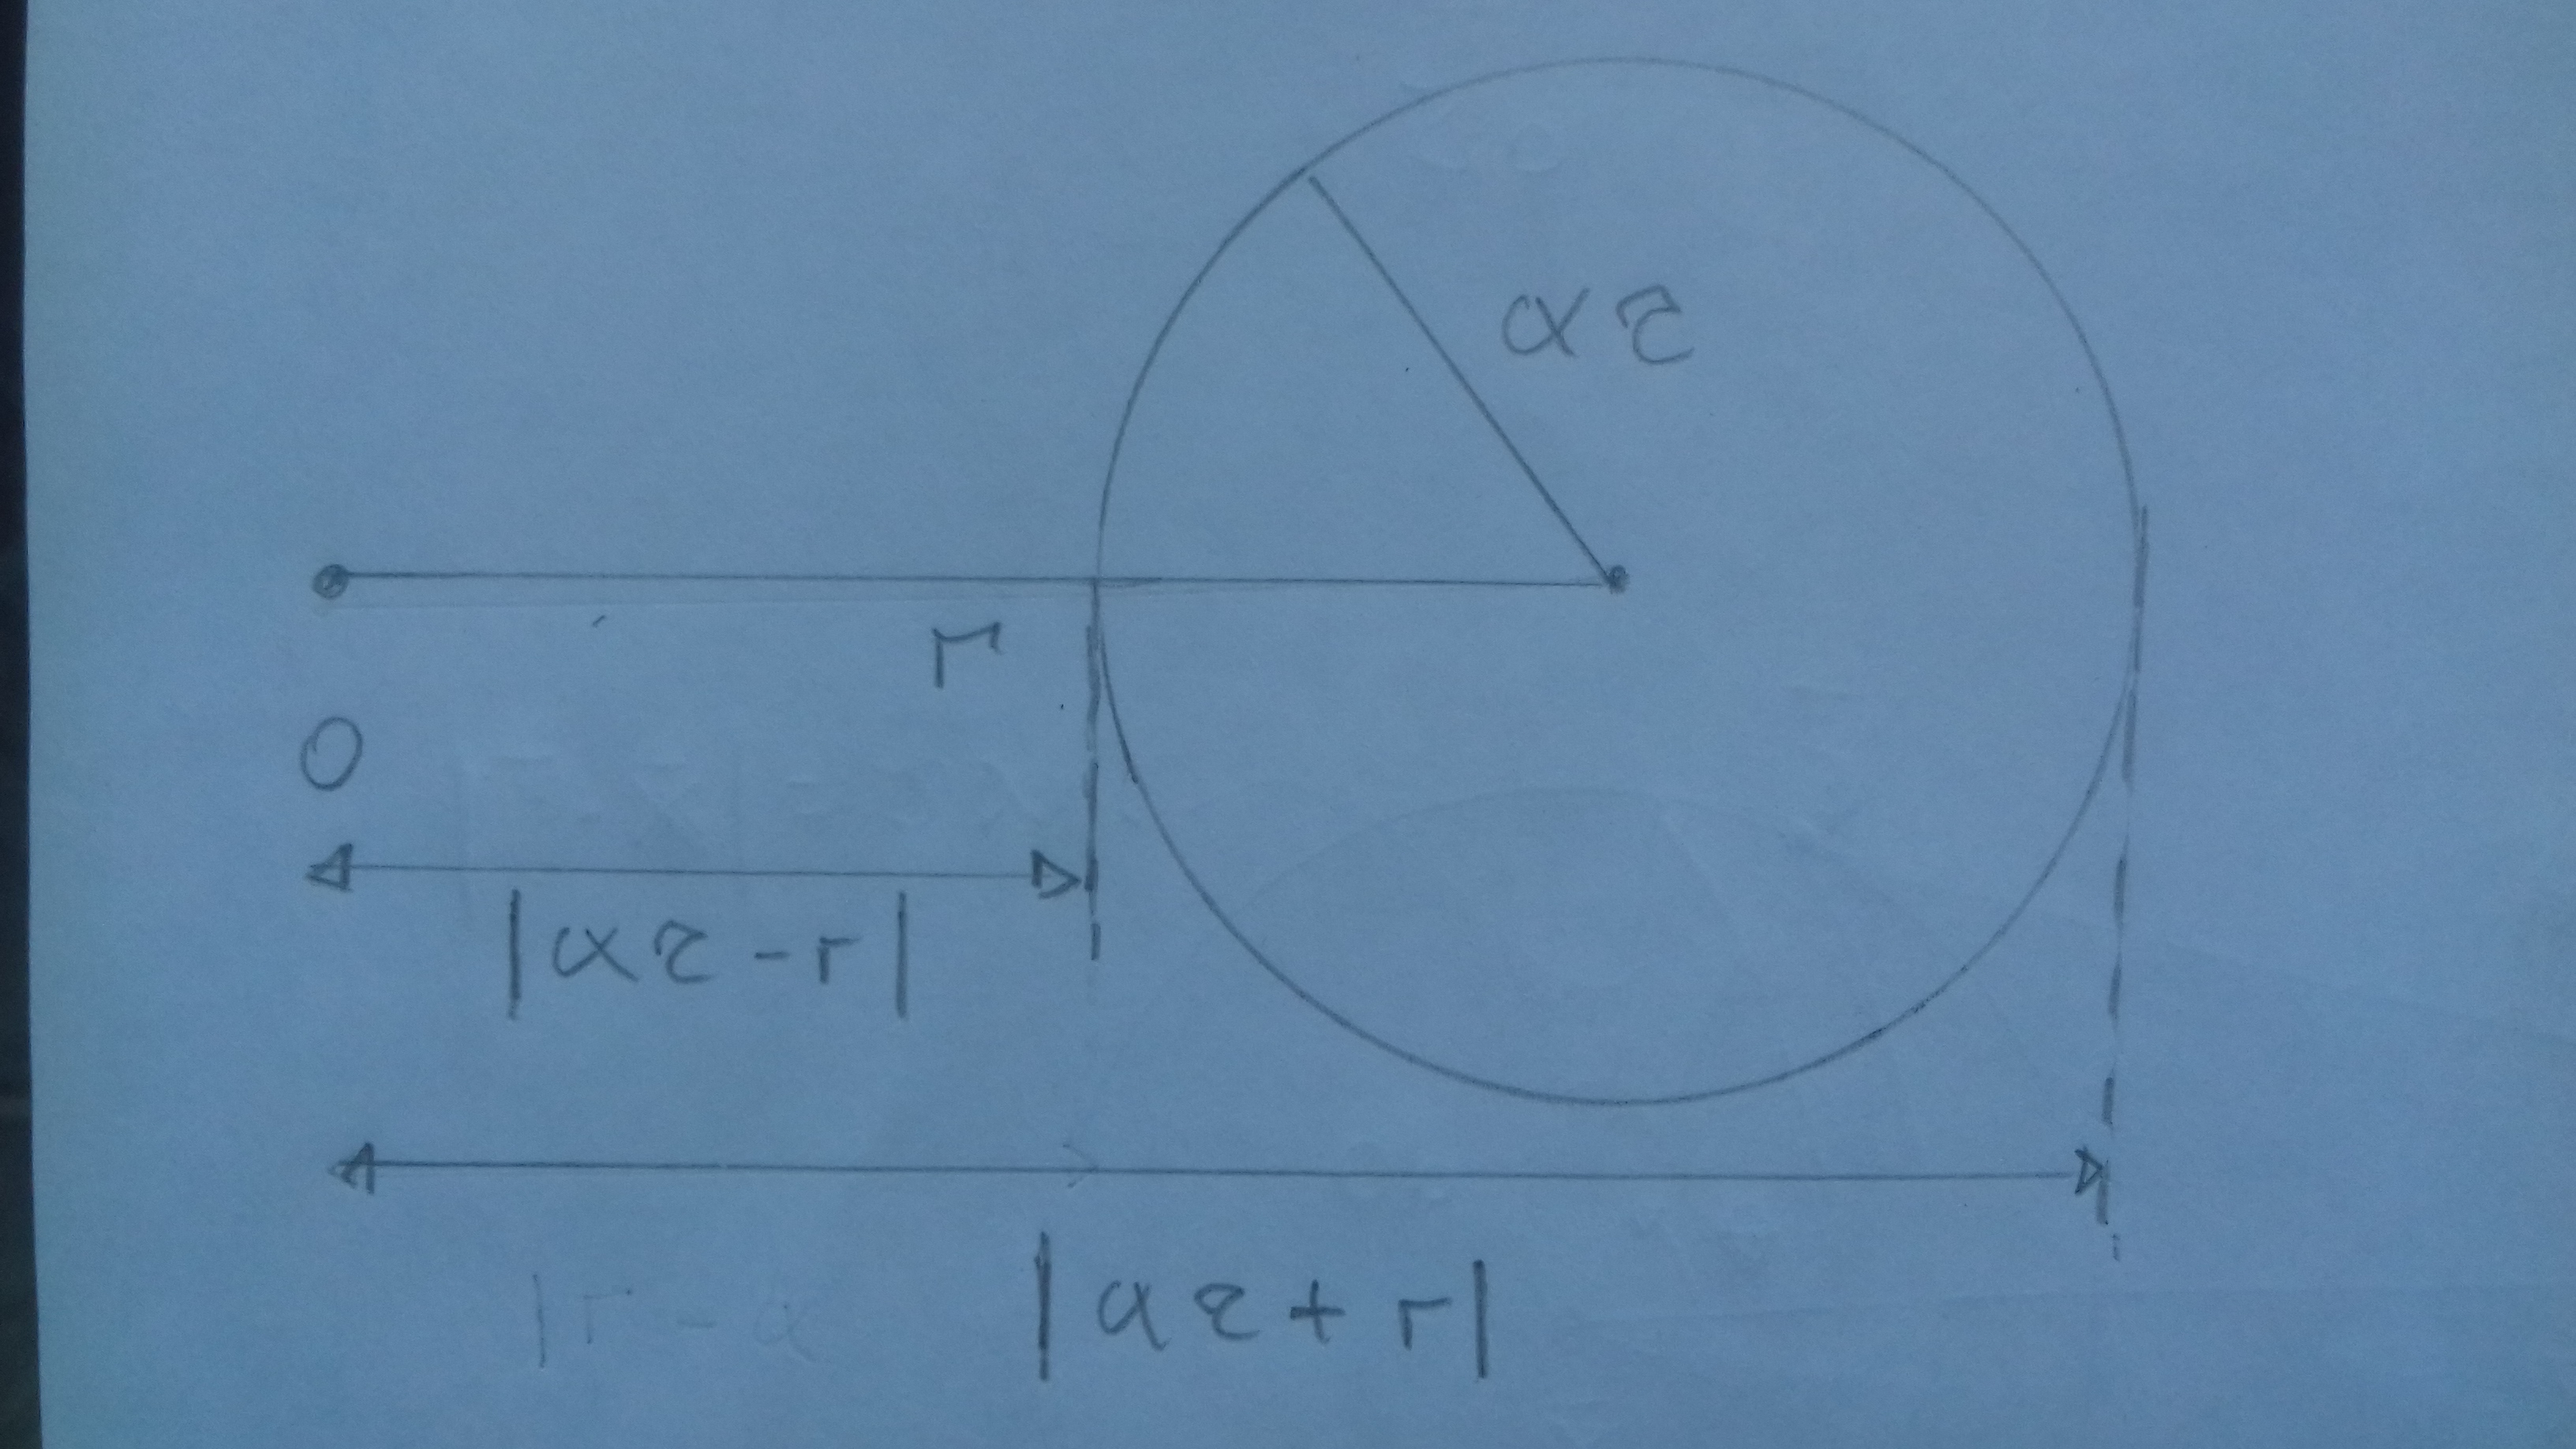
\includegraphics[scale=0.06]{Fig6}       
			\end{figure}
		\end{column}
	\end{columns}
	
	\begin{flushleft}
		Agora avaliamos a origem $O$, 
	\end{flushleft}
	\begin{eqnarray}
	\label{ten1}
	\int_{S} \frac{1}{R} dS(\eta)  &=& \frac{2\pi \alpha \tau}{r} \int_{\left| \alpha\tau -r \right|}^{\left| \alpha\tau +r \right|}  dR  = \frac{2\pi \alpha \tau}{r}\, R \Big|_{\left| \alpha\tau -r \right|}^{\left| \alpha\tau +r \right|} \, 
	\end{eqnarray}
	
\end{frame}%%%%%%%%%%%%%%%%%%%%%%%%%%%%%%%%%%%%%%%%555



\begin{frame}
	\frametitle{\textbf{Solu\c{c}\~ao para a fun\c{c}\~ao de Green em um meio homog\^eneo, isotr\'opico e ilimitado}}
	\begin{flushleft}
		\textcolor{red!60!black}{Avaliando a integral de superf\'icie:}
	\end{flushleft}
	
	\begin{flushleft}
		Agora avaliamos a origem $O$, 
	\end{flushleft}
	\begin{eqnarray}
	\label{ten1}
	\int_{S} \frac{1}{R} dS(\eta)  &=& \frac{2\pi \alpha \tau}{r} \int_{\left| \alpha\tau -r \right|}^{\left| \alpha\tau +r \right|}  dR  = \frac{2\pi \alpha \tau}{r}\, R \Big|_{\left| \alpha\tau -r \right|}^{\left| \alpha\tau +r \right|} \, 
	\end{eqnarray}
	
	\begin{itemize}
		\item Se $O$ est\'a dentro de $S$ ($ r/\alpha < \tau $):
		\begin{eqnarray}
		\label{ten1}
		\int_{S} \frac{1}{R} dS &=& \frac{2\pi \alpha \tau}{r}\left[\alpha \tau +r - (\alpha \tau -r )  \right] = 4\pi \alpha \tau
		\end{eqnarray}
		\item Se $O$ est\'a fora de $S$ ($  \tau < r/\alpha $):
		\begin{eqnarray}
		\label{ten1}
		\int_{S} \frac{1}{R} dS &=& \frac{2\pi \alpha \tau}{r}\left[\alpha \tau +r - (-\alpha \tau + r )  \right] = \frac{4\pi \alpha^2 \tau^2}{r} 
		\end{eqnarray}
	\end{itemize}
	
\end{frame}%%%%%%%%%%%%%%%%%%%%%%%%%%%%%%%%%%%%%%%%555





\begin{frame}
	\frametitle{\textbf{Solu\c{c}\~ao para a fun\c{c}\~ao de Green em um meio homog\^eneo, isotr\'opico e ilimitado}}
	\begin{flushleft}
		\textcolor{red!60!black}{Avaliando a integral de superf\'icie:}
	\end{flushleft}
	
	\begin{itemize}
		\item Se $O$ est\'a dentro de $S$ ($ r/\alpha < \tau $):
		\begin{eqnarray}
		\label{ten1}
		h &=& \frac{\partial}{\partial \eta_1} \left(  4\pi \alpha \tau \right) = 0\, 
		\end{eqnarray}
		\item Se $O$ est\'a fora de $S$ ($  \tau < r/\alpha $):
		\begin{eqnarray}
		\label{ten1}
		h &=& \frac{\partial}{\partial \eta_1} \left(  \frac{4\pi \alpha^2 \tau^2}{r} \right) =  4\pi \alpha^2 \tau^2 \frac{\partial}{\partial x_1} \frac{1}{r}\ .   
		\end{eqnarray}
	\end{itemize}
	
\end{frame}%%%%%%%%%%%%%%%%%%%%%%%%%%%%%%%%%%%%%%%%555



\begin{frame}
	\frametitle{\textbf{Solu\c{c}\~ao para a fun\c{c}\~ao de Green em um meio homog\^eneo, isotr\'opico e ilimitado}}
	
	\begin{flushleft}
		Finalmente a integral de superf\'icie tem solu\c{c}\~ao da forma:
	\end{flushleft}
	\begin{align*}
	\int_{S} \frac{\partial}{\partial x_1 } \frac{1}{\left| \xvec \right| }dS =\begin{cases}
	0  &\mbox{para}\quad  r/\alpha < \tau\\
	4\pi \alpha^2 \tau^2 \frac{\partial }{\partial x_1} \frac{1}{|\xvec|}  &\mbox{para}\quad \tau < r/\alpha
	\end{cases}
	\end{align*}
	
	\begin{flushleft}
		Assim, re-escrevemos as solu\c{c}\~oes das equa\c{c}\~oes do potencial escalar de onda P e 
		do potencial vetorial de onda S, respectivamente: 
	\end{flushleft}
	\begin{eqnarray}
	\label{ten1}
	\phi(\xvec,t) &=& - \frac{1}{4\pi \rho}  \left( \frac{\partial }{\partial x_1} \frac{1}{\left| \xvec\right|} \right)  \int_{0}^{\frac{\left| \xvec\right|}{\alpha}} \tau X_{0}\left( t -\tau \right)  d\tau\, \\
	\psi(\xvec,t) &=& \frac{1}{4\pi\rho}  \left(0, \frac{\partial }{\partial x_3} \frac{1}{\left| \xvec \right|}, -\frac{\partial }{\partial x_2} \frac{1}{\left| \xvec \right|} \right) \int_{0}^{\frac{\left| \xvec\right|}{\beta}} \tau X_{0}\left( t -\tau \right)  d\tau\, 
	\end{eqnarray}
	
\end{frame}%%%%%%%%%%%%%%%%%%%%%%%%%%%%%%%%%%%%%%%%555


\begin{frame}
	\frametitle{\textbf{Solu\c{c}\~ao para a fun\c{c}\~ao de Green em um meio homog\^eneo, isotr\'opico e ilimitado}}
	
	\begin{flushleft}
		Encontrados os potenciais de Lam\'e $\phi(\xvec,t)$ e $\psi(\xvec,t)$, podemos obter o deslocamento $\uvec(\xvec,t)$ para uma 
		fonte do tipo $X_{0}(t)\delta(\xvec)\evec_1$:
	\end{flushleft}
	\begin{eqnarray}
	\label{ten1}
	\uvec(\xvec,t) &=& \nabla \phi(\xvec,t) + \nabla \times \psi(\xvec,t)\, \\
	&=& \nabla \left[ - \frac{1}{4\pi \rho}  \left( \frac{\partial }{\partial x_1} \frac{1}{\left| \xvec\right|} \right)  \int_{0}^{\frac{\left| \xvec\right|}{\alpha}} \tau X_{0}\left( t -\tau \right)  d\tau  \right] \, \\
	&=& \nabla \times \left[ \frac{1}{4\pi\rho}  \left(0, \frac{\partial }{\partial x_3} \frac{1}{\left| \xvec \right|}, -\frac{\partial }{\partial x_2} \frac{1}{\left| \xvec \right|} \right) \int_{0}^{\frac{\left| \xvec\right|}{\beta}} \tau X_{0}\left( t -\tau \right)  d\tau\right] \, .
	\end{eqnarray}
	
\end{frame}%%%%%%%%%%%%%%%%%%%%%%%%%%%%%%%%%%%%%%%%555


\begin{frame}
	\frametitle{\textbf{Solu\c{c}\~ao para a fun\c{c}\~ao de Green em um meio homog\^eneo, isotr\'opico e ilimitado}}
	
	\begin{flushleft}
		Encontrados os potenciais de Lam\'e $\phi(\xvec,t)$ e $\psi(\xvec,t)$, podemos obter o deslocamento $\uvec(\xvec,t)$ para uma 
		fonte do tipo $X_{0}(t)\delta(\xvec)\evec_1$:
	\end{flushleft}
	\begin{eqnarray}
	\label{ten1}
	u_i(\xvec,t) &=& 
	\frac{1}{4\pi \rho}  \left( \frac{\partial^2 }{\partial x_i \partial x_1} \frac{1}{r } \right)  \int_{ \frac{r }{\alpha}}^{ \frac{r}{\beta}} \tau X_{0} \left( t -\tau \right)  d\tau\, \\      
	&+& \frac{1}{4\pi \alpha^2 \rho} \frac{1}{r}  \left(\frac{\partial r}{ \partial x_i} \frac{\partial r}{ \partial x_1}  \right)  X_{0} \left(t - \frac{r}{\alpha} \right) \\
	&+& \frac{1}{4\pi\beta^2 \rho} \left( \delta_{i1}  -  \frac{\partial r}{ \partial x_i} \frac{\partial r}{ \partial x_1}  \right) X_{0} \left(t - \frac{r}{\beta} \right)  \, ,
	\end{eqnarray}
	onde $r = \left| \xvec \right|$.
	
\end{frame}%%%%%%%%%%%%%%%%%%%%%%%%%%%%%%%%%%%%%%%%555


\begin{frame}
	\frametitle{\textbf{Solu\c{c}\~ao para a fun\c{c}\~ao de Green em um meio homog\^eneo, isotr\'opico e ilimitado}}
	
	\begin{flushleft}
		Co-senos directores $\gamma_i= (\gamma_1,\gamma_2,\gamma_3)$ para o vetor $\xvec = (x_1,x_2,x_3)$, 
	\end{flushleft}
	\begin{equation}
	\gamma_1 = \frac{\xvec \cdot \evec_1}{r \left| \evec_1 \right|} = \frac{(x_1,x_2,x_3) \cdot (1,0,0)}{r} = \frac{x_1}{r}
	\end{equation}
	\begin{flushleft}
		e observe que
	\end{flushleft}
	\begin{equation}
	\frac{\partial r}{\partial x_1} = \frac{\partial }{\partial x_1}\left( \sqrt{x_1^2 + x_2^2 + x_3^2} \right)   =  \frac{x_1}{\sqrt{x_1^2 + x_2^2 + x_3^2}} =  \frac{x_1}{r}
	\end{equation}
	\begin{flushleft}
		Assim,
	\end{flushleft}
	\begin{equation}
	y_i = \frac{x_i}{r} = \frac{\partial r}{\partial x_i}  
	\end{equation}
	\begin{flushleft}
		De forma an\'aloga, a derivada de $r^{-1}$ em rela\c{c}\~ao $x_j$ e depois em $x_i$ \'e
	\end{flushleft}
	\begin{equation}
	\frac{\partial^2}{\partial x_i \partial x_j} \frac{1}{r}  = \frac{3\gamma_i\gamma_j - \delta_{ij}}{r^3}\, .
	\end{equation}
	
\end{frame}%%%%%%%%%%%%%%%%%%%%%%%%%%%%%%%%%%%%%%%%555


\begin{frame}
	\frametitle{\textbf{Solu\c{c}\~ao para a fun\c{c}\~ao de Green em um meio homog\^eneo, isotr\'opico e ilimitado}}
	
	\begin{flushleft}
		\textbf{Solu\c{c}\~ao de Stokes (1849)}: tomando $X_{0}(t)$ como uma for\c{c}a pontual atuando na dire\c{c}\~ao $x_j$ na origem e usando os co-senos 
		directores,
	\end{flushleft}
	\begin{eqnarray*}
		\label{ten1}
		u_i(\xvec,t) &=& X_{0}(t) * G_{ij}(\xvec,t;\xivec,0)\, \\
		&=&\frac{1}{4\pi\rho} \left(3\gamma_i\gamma_j -\delta_{ij} \right) \frac{1}{r^3}  \int_{ \frac{r }{\alpha}}^{ \frac{r}{\beta}} \tau X_{0}\left( t -\tau \right)  d\tau\, \\      
		&+&\frac{1}{4\pi\alpha^2\rho} \gamma_i\gamma_j \,\frac{1}{r}  X_{0}\left(t - \frac{r}{\alpha} \right)\, \\
		&-&\frac{1}{4\pi\beta^2\rho} \left(\gamma_i\gamma_j -\delta_{ij} \right)  \frac{1}{r}  X_{0}\left(t - \frac{r}{\beta} \right)\, .
	\end{eqnarray*}
	\begin{flushleft}
	\end{flushleft}
\end{frame}%%%%%%%%%%%%%%%%%%%%%%%%%%%%%%%%%%%%%%%%555



\begin{frame}
	\frametitle{\textbf{Solu\c{c}\~ao para a fun\c{c}\~ao de Green em um meio homog\^eneo, isotr\'opico e ilimitado}}
	
	\begin{flushleft}
		\textbf{Solu\c{c}\~ao de Stokes (1849)}: tomando $X_{0}(t)$ como uma for\c{c}a pontual atuando na dire\c{c}\~ao $x_j$ na origem e usando os co-senos 
		directores,
	\end{flushleft}
	\begin{eqnarray*}
		\label{ten1}
		u_i(\xvec,t) &=& X_{0}(t) * G_{ij}(\xvec,t;\xivec,0)\, \\
		&=&\frac{1}{4\pi\rho} \textcolor{red}{\left(3\gamma_i\gamma_j -\delta_{ij} \right) \frac{1}{r^3}  \int_{ \frac{r }{\alpha}}^{ \frac{r}{\beta}} \tau X_{0}\left( t -\tau \right)  d\tau }\, \\      
		&+&\frac{1}{4\pi\alpha^2\rho} \gamma_i\gamma_j \,\frac{1}{r}  X_{0}\left(t - \frac{r}{\alpha} \right)\, \\
		&-&\frac{1}{4\pi\beta^2\rho} \left(\gamma_i\gamma_j -\delta_{ij} \right)  \frac{1}{r}  X_{0}\left(t - \frac{r}{\beta} \right)\, .
	\end{eqnarray*}
	\begin{flushleft}
		\textcolor{red}{Near-field de modo P e S}
	\end{flushleft}
\end{frame}%%%%%%%%%%%%%%%%%%%%%%%%%%%%%%%%%%%%%%%%555


\begin{frame}
	\frametitle{\textbf{Solu\c{c}\~ao para a fun\c{c}\~ao de Green em um meio homog\^eneo, isotr\'opico e ilimitado}}
	
	\begin{flushleft}
		\textbf{Solu\c{c}\~ao de Stokes (1849)}: tomando $X_{0}(t)$ como uma for\c{c}a pontual atuando na dire\c{c}\~ao $x_j$ na origem e usando os co-senos 
		directores,
	\end{flushleft}
	\begin{eqnarray*}
		\label{ten1}
		u_i(\xvec,t) &=& X_{0}(t) * G_{ij}(\xvec,t;\xivec,0)\, \\
		&=&\frac{1}{4\pi\rho} \textcolor{red}{\left(3\gamma_i\gamma_j -\delta_{ij} \right) \frac{1}{r^3}  \int_{ \frac{r }{\alpha}}^{ \frac{r}{\beta}} \tau X_{0}\left( t -\tau \right)  d\tau }\, \\      
		&+&\frac{1}{4\pi\alpha^2\rho} \textcolor{blue}{\gamma_i\gamma_j\, \frac{1}{r}  X_{0}\left(t - \frac{r}{\alpha} \right) }\, \\
		&-&\frac{1}{4\pi\beta^2\rho} \left(\gamma_i\gamma_j -\delta_{ij} \right)  \frac{1}{r}  X_{0}\left(t - \frac{r}{\beta} \right)\, .
	\end{eqnarray*}
	\begin{flushleft}
		\textcolor{red}{Near-field de modo P e S}\hspace{0.5cm}
		\textcolor{blue}{Far-field de onda P}
	\end{flushleft}
\end{frame}%%%%%%%%%%%%%%%%%%%%%%%%%%%%%%%%%%%%%%%%555


\begin{frame}
	\frametitle{\textbf{Solu\c{c}\~ao para a fun\c{c}\~ao de Green em um meio homog\^eneo, isotr\'opico e ilimitado}}
	
	\begin{flushleft}
		\textbf{Solu\c{c}\~ao de Stokes (1849)}: tomando $X_{0}(t)$ como uma for\c{c}a pontual atuando na dire\c{c}\~ao $x_j$ na origem e usando os co-senos 
		directores,
	\end{flushleft}
	\begin{eqnarray*}
		\label{ten1}
		u_i(\xvec,t) &=& X_{0}(t) * G_{ij}(\xvec,t;\xivec,0)\, \\
		&=&\frac{1}{4\pi\rho} \textcolor{red}{\left(3\gamma_i\gamma_j -\delta_{ij} \right) \frac{1}{r^3}  \int_{ \frac{r }{\alpha}}^{ \frac{r}{\beta}} \tau X_{0}\left( t -\tau \right)  d\tau }\, \\      
		&+&\frac{1}{4\pi\alpha^2\rho} \textcolor{blue}{\gamma_i\gamma_j\, \frac{1}{r}  X_{0}\left(t - \frac{r}{\alpha} \right) }\, \\
		&-&\frac{1}{4\pi\beta^2\rho} \textcolor{green}{\left(\gamma_i\gamma_j -\delta_{ij} \right)  \frac{1}{r}  X_{0}\left(t - \frac{r}{\beta} \right) }\, .
	\end{eqnarray*}
	\begin{flushleft}
		\textcolor{red}{Near-field de modo P e S} \hspace{0.5cm}
		\textcolor{blue}{Far-field de onda P}\hspace{0.5cm}
		\textcolor{green}{Far-field de onda S}
	\end{flushleft}
\end{frame}%%%%%%%%%%%%%%%%%%%%%%%%%%%%%%%%%%%%%%%%555



%%%%%%%%%%%%%%%%Lucas%%%%%%%%%%%%%%%%%%
\section{Propriedades do \textit{far-field}}

%%%%%%%%%%Onda P
\begin{frame}{Propriedades do \textit{far-field} para onda $P$}
\visible<1->{	Deslocamento $\vc{u}^P$ é dado por
	$$u_i^P(\vc{x},t)= \frac{1}{4\pi \rho \alpha ^2}\gamma_i\gamma_j\frac{1}{r}X_0\left(t-\frac{r}{\alpha}\right)$$}
\begin{enumerate}
	\justifying
\visible<2->{\item Atenua com $r^{-1}$; }
\visible<3->{\item Forma da onda;}
\visible<4->{\item Propaga com a velocidade $\alpha$($\alpha^2 = (\lambda +2\mu)/\rho$);}
\visible<5->{\item Forma da onda de deslocamento;}
\visible<6->{\item Direção de deslocamento $\vc{u}^P$ em $\vc{x}$ é paralela a direção $\vc{\gamma}$ da fonte.}	
\end{enumerate}
\end{frame}
%%%%%%%%%%Onda S
\begin{frame}{Propriedades do \textit{far-field} para onda $S$}
\visible<1->{	Deslocamento $\vc{u}^S$ é dado por
	$$u_i^S(\vc{x},t)= \frac{1}{4\pi \rho \beta ^2}(\delta_{ij}-\gamma_i\gamma_j)\frac{1}{r}X_0\left(t-\frac{r}{\beta}\right)$$}
\begin{enumerate}
	\justifying
	\visible<2->{\item Atenua com $r^{-1}$; }
	\visible<4->{\item Propaga com a velocidade $\beta$;}
	\visible<5->{\item Forma da onda de deslocamento;}
	\visible<6->{\item Direção de deslocamento $\vc{u}^S$ em $\vc{x}$ é perpendicular a direção $\vc{\gamma}$ da fonte.}	
\end{enumerate}
	
\end{frame}
%%%%%%%%%Figura radiação
\begin{frame}{Padrões de radiação de $\vc{u}^P$ e $\vc{u}^S$}
		\begin{figure}[htb]
		\centering
		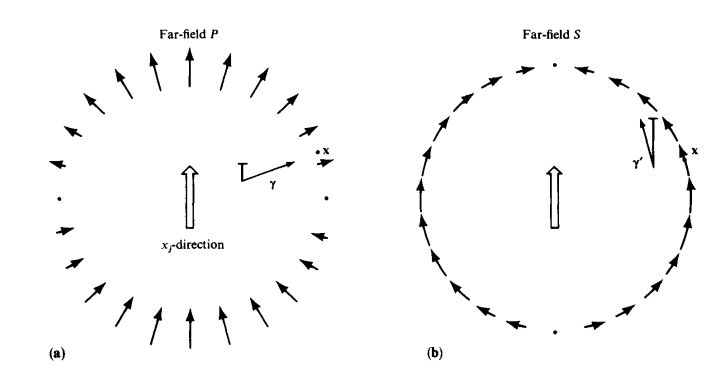
\includegraphics[width= 10cm, height= 8cm]{radiacao}
	\end{figure}
\end{frame}

%%%%%%%%%%%%%%%%Amanda%%%%%%%%%%%%%%%%%
\section{Propriedades do \textit{near-field}}

\begin{frame}
	
	\frametitle {Propriedades dos termos do Near-Field}
	
	\begin{itemize}
		\item Definimos o campo de deslocamento próximo $u^{N}$ por:
	\end{itemize}
	
	\begin{equation}
	u_{i}^{N}(x,t)= \frac{1}{4\pi\rho}(3\gamma_{i}\gamma_{j}-\delta_{ij})\frac{1}{r^{3}} \int_{r/\alpha}^{r/\beta} \tau X_{0}(t-\tau) \,d\tau\ .
	\end{equation}
	
	\begin{figure}
		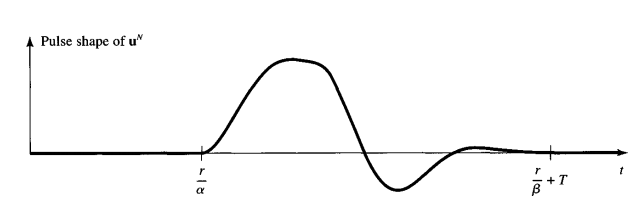
\includegraphics[scale=1.5]{fig1.png}
	\end{figure}
	
	
\end{frame}

\begin{frame}
	\begin{itemize}
		\item componente longitudinal
		
		\begin{equation}
		u^{N}.\gamma= \gamma _{j}\frac{1}{2\pi\rho r^{3}}\int_{r/\alpha}^{r/\beta} \tau X_{0}(t-\tau) \,d\tau\ .
		\end{equation}
		
		\item componente transversal
		\begin{equation}
		u^{N}.\gamma^{'}= -\gamma^{'} _{j}\frac{1}{4\pi\rho r^{3}}\int_{r/\alpha}^{r/\beta} \tau X_{0}(t-\tau) \,d\tau\ .
		\end{equation}
	\end{itemize}
	
	
\end{frame}

\begin{frame}
	\frametitle {Near-Field (Campos próximos)}
	\begin{itemize}
		\item Para o deslocamento Near-Field, não é possível identificar as propriedades simples como nos campos distantes; 
		\item Podemos identificar o tempo de transito e a duração do deslocamento em um receptor fixo;
		\item A duração do movimento do campo de deslocamento Near Field é igual a diferença entre os tempos de transitos das ondas P e S mais o termo T.
	\end{itemize}
\end{frame}

\section{Caso para o tensor de momento}

\begin{frame}{Caso para o tensor de momento}
	\small
	\begin{eqnarray}
	M_{pq} \ast G_{np,q} &=&\textcolor{red}{\left(\frac{15\gamma_n\gamma_p\gamma_q-3\gamma_n\delta_{pq}-3\gamma_p\delta_{nq}-3\gamma_{q}\delta_{np}}{4\pi\rho}\right)\frac{1}{r^4}\int_{r/\alpha}^{r/\beta} \tau M_{pq}(t-\tau) d\tau} \nonumber \\
	&&+ \textcolor{orange}{\left(\frac{6\gamma_n\gamma_p\gamma_q-\gamma_n\delta_{pq}-\gamma_p\delta_{nq}-\gamma_{q}\delta_{np}}{4\pi\rho\alpha^2}\right)\frac{1}{r^2}M_{pq}\left(t-\frac{r}{\alpha}\right)} \nonumber \\
	&&-
	\textcolor{orange}{\left(\frac{6\gamma_n\gamma_p\gamma_q-\gamma_n\delta_{pq}-\gamma_p\delta_{nq}-\gamma_{q}\delta_{np}}{4\pi\rho\beta^2}\right)\frac{1}{r^2}M_{pq}\left(t-\frac{r}{\beta}\right)} \nonumber \\
	&&+\textcolor{blue}{ \frac{\gamma_n \gamma_p \gamma_q}{4\pi\alpha^3}\frac{1}{r}\dot{M}_{pq}\left(t-\frac{r}{\alpha}\right)}- \textcolor{green}{\left(\frac{\gamma_n\gamma_p-\delta_{np}}{4\pi\beta^3}\right)\gamma_{q}\frac{1}{r}\dot{M}_{pq}\left(t-\frac{r}{\beta}\right)} \nonumber
	\end{eqnarray}
	\begin{flushleft}
		\textcolor{red}{Near-field de modo P e S} \hspace{0.5cm}
		\textcolor{blue}{Far-field de onda P}\hspace{0.5cm}
		\textcolor{green}{Far-field de onda S}
	\end{flushleft}
    \begin{center}
    	\textcolor{orange}{Termos intermediários}
    \end{center}
\end{frame}

\end{document}